\section{Úvod} % (fold)
\label{sec:_vod}

% Postupom času sa vyvinuli rôzne spôsoby ako prispôsobiť web aj na mobilné zariadenia. Medzi najpoužívanejšia techniky patria ,,\textit{Responsive design}'', ,,\textit{Mobile-first responsive design}'', ,,\textit{Progressive enhancement}'' a ,,\textit{Server-side adaptation}''\cite{mobiforge} .

% Najlepší spôsob prispôsobenia obsahu je však taký, ktorý pokrýva všetky zariadenia od najmenších mobilných po veľké televízne obrazovky a nevytvára pre rôzne zariadenia vlastné stránky. Tieto podmienky z časti spĺňa technika ,,\textit{Mobile-first responsive design}'' založená na používaní flexibilného vzhľadu stránky, flexibilných obrázkov a media queries \cite{responsive, mediaqueries}, pričom sa postupuje aj od malých zariadení k veľkým obrazovkám. Táto technika však nemusí byť vždy úplne postačajúca, a preto sa hodí využiť kombináciu rôznych spôsobov.

Web sa neustála vyvíja a my sa musíme prispôsobiť. S príchodom mobilných zariadení, ktoré postupne nahradzujú klasické počítače, vznikol problém pri správnom zobrazovaní webového obsahu. Web na ne nebol pripravený, a tak sa im ponúkala verzia stránky pre klasické počítače. Dnes však neriešime web len stolové počítače, ale aj pre mobilné zariadenie, tablety, televízie, nositeľné prístroje a ďalšie. Aj veci pre priemernú webovú stránku ako sú podieľ prehliadačov, operačných systémov či rozlíšení sa za posledné roky v mnohom zmenili \cite{ui17}.

Len za posledných pár rokov sa vo svete predalo viac ako 1 bilión mobilných zariadení, 1.038 bilióna celkovo \cite{bilion}. Mobilné telefóny a tablety sa stali ešte viac personálnymi a používajú sa neustále počas celého dňa pri rôznych činnostiach \cite{mobileuse, smarthopenseveryday, tabletuse}. Ich predajnosť sa zvýšuje každým dňom. V porovnaní vývoja trhového podielu osobných počítačov typu WINTEL a mobilných zariadení Apple a Android za posledné roky je tento trend ešte viac viditeľný.

Postupom času sa vyvinuli rôzne spôsoby ako prispôsobiť web aj na mobilné zariadenia. Najlepší spôsob prispôsobenia obsahu je taký, ktorý pokrýva všetky zariadenia od najmenších mobilných po veľké televízne obrazovky a nevytvára pre rôzne zariadenia vlastné samostané stránky.

Ignorovanie webu na mobilných zariadeniach väčšinou spoločností však vedie k vytváraniu samostatných natívnych aplikácii pre každú platformu. Okrem vedúceho postavenia Androidu a iOS existuje množstvo ďalších platforiem, pre ktorú treba vytvoriť vlastnú aplikáciu, a tým sa vývoj predražuje. Nevýhodou natívnych aplikácii je, že neotvárajú webové odkazy a stále nemáme istotu, že si ich používateľ stiahne a nainštaluje. Taktiež vzniká problém pri aktualizáciách, používateľ ju músí manuálne spustiť. Nestačí len otvoriť aplikáciu, ktorá bude automaticky obsahovať najnovšiu verziu ako web. S tým je spojený aj problém s ich udržiavaním.

Práve tu je neoddeliteľná súčasť webu a mobilných zariadení. V súčasnosti populárne sociálne siete, ale aj emaily či qr kódy obsahujú množstvo odkazov na web. Na rovnaké odkazy je však možné pristúpiť aj z klasických počítačov. Je tak dôležité, aby sa obsah používateľom zobrazil správne bez ohľadu na to, na akom zariadení k nemu pristupujú.

Optimalizácia webového obsahu pre mobilné zariadenia má veľmi krátku históriu. Dnes však už existujú základné vzory, podľa ktorých je možné prispôsobiť zobrazenie webového obsahu na ich malé displeje \cite{mobilebookpatterns, navigation}. Problémom je, že neustále rastú rozmery mobilných zariadení, ale aj veľké televízne obrazovky sa stávajú prístupovým bodom k webovému obsahu. Len za posledné 3 mesiace bolo predaných 29\% android zariadení s obrazovkou väčšou ako 4.5 palca \cite{bigscreen} a k podobnému trendu pristupujú aj iní výrobcovia.

Optimalizácia webového obsahu zariadeniam však neznamená len jeho vizuálne prispôsobene rôznym veľkostiam displejom. Nemenej dôležitým prvkom je aj pripojiteľnesť zariadenia na sieť s cieľom čo najrýchlejšieho stihnutia, zobrazenia stránky a šetrenia používateľových prenášaných dát a financií. Nielen práve preto je vhodné použiť princípy adaptívneho web dizajnu. Medzi jeho hlavné charakteristiky patria všadeprítomnosť, flexibilita, výkonnosť, rozšíriteľnosť a priateľskosť k budúcnosti \cite{adaptive}. V súčasnosti nevieme povedať aké zariadenia sa budú predávať o pár rokov, aké budú mať vlastnosti, ale s celkom veľkou pravdepodobnosťou budú obsahovať webový prehliadač. 

Adaptívny web dizajn je v podstate ,,Progressive enhancement'', len je aplikovaný na mnoho širšie a diverzifikovanejšie spektrum. Pripojenie na internet sa v súčasnosti nachádza na smartfónoch, tabletoch, e-čítačkach, netbookoch, hodinkách, televízoroch, phabletoch, notebookoch, herných konzolách, autách a na mnohých iných zariadeniach. Taktiež máme mnoho druhov internetových pripojení s rozdielnými rýchlosťami, latenciami či kvalitou. ,,Responzívny Web dizajn'' je taktiež jednou z techník používanou v stretégii adaptívneho web dizajnu. Vytváranie flexibilných rozvrhnutí stránok je dôležité, ale je tu ešte mnoho ďalších faktorov na ktoré musíme myslieť. Je dôležité brať do úvahy ergonómiu, možnosti dotyku či iných interakčných metód, internetové pripojenie a množstvo ďalších faktorov, ktoré vieme detekovať.

Adaptívny web dizajn považujeme za zhodný s vytvorením jednotného webového zážitku. Môžme ho pripôsobiť na základe možností ponúkaných konkrétnym zariadením či prehliadačom. Webové aplikácie môžu pristúpiť k senzorom v zariadeniach a použiť ich na zlepšenie používateľského zážitku.

Výzvou sa tak stáva nie len vytvorenie celkového používateľského rozhrania, ale aj jednotlivých prvkov ako je navigácia či ovládacie prvky, ktoré by pomohli správne zobraziť obsah na malých zariadeniach a zároveň aby sa obsah prispôsobil aj tabletom, klasickým počítačom či pre veľké obrazovky televíznych príjmačov. Keďže rozlíšenia mobilných zariadení sa začínajú prelínať s klasickými počítačmi a aj klasické počítače pridávajú nové spôsoby ovládania dotykom, je dôležité rozoznať spôsob ovládania zariadenia a prispôsobiť navigáciu a obsah na dotyk alebo klávesnicu a myš. Rovnako je potrebné rozoznať aj internetové pripojenie zariadenia a automaticky mu odovzdať taký obsah, aby sa mu čo najrýchlejšie načítal a aby to používateľa nestálo zbytočný čas a financie za prenášané dáta.



% section _vod (end)


% section adapta_n_techniky (end)

\section{Adaptácia webových aplikácií} % (fold)
\label{sec:adapt_cia}

\subsection{Možnosti prispôsobenia} % (fold)
\label{sub:mo_nosti_prisp_sobenia}

Existuje mnoho možností, na základe ktorých môžme prispôsobovať webové aplikácie jednotlivým zariadeniam. Hlavným prvkom adaptácie je veľkosť a rozlíšenie displeja cieľového zariadenia. Ďalšími ale nemej dôležitými sú spôsoby ovládania zariadenia, jeho pripojenie na internet alebo samotná platforma.

\subsubsection{Veľkosť a rozlíšenie} % (fold)
\label{ssub:ve_kos_a_rozl_enie}

Jednou zo základných možností prispôsobenia webových aplikácii je adaptácia na základe zobrazovacieho displeja zariadenia. Displeje môžu mať rozličné fyzické veľkosti ale aj rozlíšenia.

Časy s ,,rovnakým'' displejom na všetkých zariadeniach a podporou jednotného statického rozlíšenia na webových stránkach sú už dávno preč. S príchodom nových malých mobilných zariadení sa potreba prispôsobenia ešte viac umocnila. Veľkosti a rozlíšenia zariadení sa postupne začínali prelínať, dokonca v súčasnosti sa na trh uvádzajú zariadenia s väčším rozlíšením ako majú monitory stolových počítačov.


\begin{figure}[H]
	\centering
	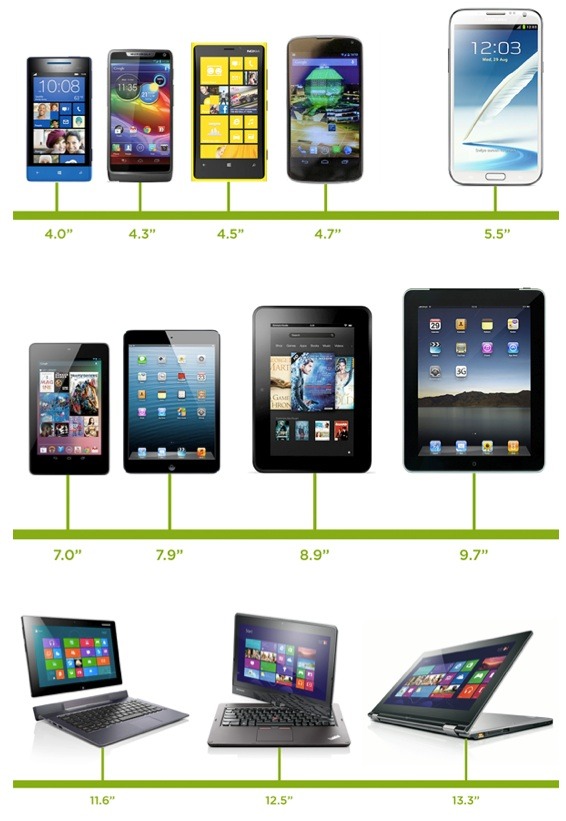
\includegraphics[width=0.75\textwidth]{img/tnav-devices.jpg}
	\caption[Porovnanie zariadení vzhľadom na veľkosť displeja]{
		Porovnanie zariadení vzhľadom na veľkosť displeja \cite{navigation}.\\
		Prevzaté z http://www.lukew.com/ff/entry.asp?1649}
	\label{fig: tnavmobile}
\end{figure}

Keďže sa začínajú vyskytovať rovnaké rozlíšenia displaja na rozlične veľkých zariadeniach alebo opačne, je potrebné medzi zariadeniami rozlíšovať aj inými spôsobmi. Je potrebné správne poruzumieť jednotkám ,,pixel'' a ,,viewport''.

Na rozdiel od pixelu definovaného W3C pomocou pozorovacieho uhlu a vzdlialenosti \cite{w3cpixel} existujú rôzne iné bežne používané jednotky ,,CSS pixel'', ,,device pixel'' a ,,density-independent pixel'' \cite{pixelnotpixel}. CSS pixel je abstrakný, môže sa zvyšovať alebo zniživať, používa sa bežne v kóde na definovanie rozmerov elementov.  Device pixel je fyzický pixel nachádzajúci sa na zariadení. Pretože zariadenia majú stále viac fyzických pixelov a tým aj ich väčsiu hustotu, zaviedol sa pojem density-independent pixel. Ten je opäť abstraktný a predstavuje počet CSS pixelov optimálnych na prezeranie obsahu. Pokiaľ by nebol zavedený, tak zariadenia s veľkou hustotou pixelov by sa nedali použiť na bežné prezeranie obsahu, nakoľku pixely sú veľmi malé a zobrazený text alebo elementy by tak boli nečitaľné.

Viewport je celkové miesto potrebné na zobrazenie webovej stránky. Na mobilných zariadeniach je situácia komplikovanejšia, pretože stále existuje množstvo stránok, ktoré nie sú na ne optimalizované. Preto ho výrobcovia mobilných prehliadačov rozdelili na ,,layout viewport'' a ,,visual viewport''. \cite{pixelnotpixel} Layout viewport je pre rozmiestnenie elementov celej stránky a visual viewport je definovaný pre elemty po priblížení stránky tak, že sa nezmestila na displej zariadenia.

% subsubsection ve_kos_a_rozl_enie (end)

\subsubsection{Interakčné prostriedky} % (fold)
\label{ssub:interak_n_prostriedky}

Postupom času začína upadať používanie klasických stolových počítačov ovládaných pomocou klávesnice a myši a presadzujú sa nové druhy mobilných zariadení so vstupným interfejsom v podobe množstva senzorov, ale hlavne s dotykovou plochou. Tá sa ako ovládací prostriedok začína presadzovať okrem mobilných zariadení aj v notebookoch. Pri dizajne aplikácie je preto potrebné myslieť aj na takýchto používateľov. Okrem nich však existujú aj iné možnosti ovládania ako sú napríklad sledovanie pohybu pomocou web kamery, natočanie a posúvanie zariadenia získané pomocou gyroskupu a accelerometra či počúvanie hlasových povelov zaznamenaných cez mikrofón. Je tak potrebné brať do úvahy aj ďalšie možnosti.

Webové prehliadače na televízoroch sú celkom dobré, ale interakcia s nimi je otrasná, tak ich nikto nepoužíva. Vstupné metódy sú tak oveľa dôležitejšie pri tvorbe dizajnu než veľkosti displejov. Vstup definuje ako musí vyzerať dizajn pre splnenie úloh \cite{adaptiveinput}. Taktiež máme na tele nositeľné zariadenia. Súčasný interfejs Google Glass je limitovaný len na pár vstupných metód.

Univerzálny interakčný prostriedok pre web neexistuje. Musíme sa rozhodovať medzi dotykom, klávesnicou, myšou, rečou a ďalšími. Výzvou pre nasledujúce roky sa stáva nedefinovať dizajn len pre jeden druh interakcie ale pre mnoho.

% \newpage

\paragraph{Dotyk} % (fold)

Dôležitým prvkom v prípade mobilných zariadení je možnosť ovládania aplikácii jednou rukou. Mobilné zariadenia sú využívané takmer pri každej príležitesti či vo vonkajšom alebo vnútornom prostredí, preto je potrebné správne prispôsobiť vzhľad a rozmiestnenie ovládacích prvkov. Pre ne platí, že najjednoduchšie dosiahnuteľné časti sú v spodnej strane zariadenia a s postupom k hornému okraju možnosť dosiahnutia klesá \cite{mobilebooktouch}.

Dotyk však už nie je izolovaný len pre mobilné zariadenia. V súčasnosti množstvo veľkých obrazoviek či notebookov disponuje dotykovým ovládaním. Teda dizajn aj pre väčšie displeje musí byť prispôsobený na dotyk. Optimálna veľkosť elementu by mala byť aspoň 7mm čo predstavuje 30 pixelov \cite{designingfortouch}. Ale veci nie sú len také jednoduché pretože existujú dynamické veľkosti displejov oproti fyzikálnym.

\begin{figure}[H]
        \centering
        \begin{subfigure}[b]{0.6\textwidth}
                \centering
                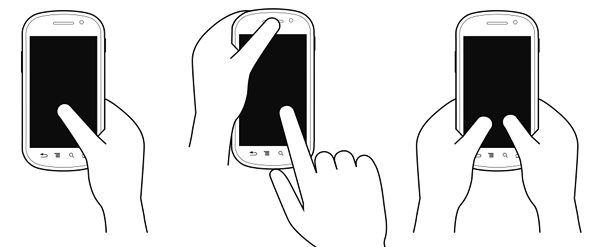
\includegraphics[width=\textwidth]{img/tnav-touch-phones.png}
        \end{subfigure}%
         %add desired spacing between images, e. g. ~, \quad, \qquad etc.
          %(or a blank line to force the subfigure onto a new line)
        \begin{subfigure}[b]{0.2\textwidth}
                \centering
                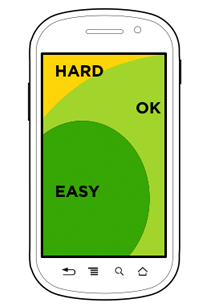
\includegraphics[width=\textwidth]{img/tnav-touch-phones2.png}
        \end{subfigure}

        \caption[Schopnosť ovládania mobilných telefónov]{Schopnosť ovládania mobilných telefónov \cite{navigation}.\\
		Prevzaté z http://www.lukew.com/ff/entry.asp?1649}
		\label{fig:tnavphones}
\end{figure}

Väčšie mobilné zariadenia alebo tablety už nie je možné pohodlne udržať v jednej ruke a tak je dôležité prispôsobiť ovládanie na dve ruky. Tablety sú držané v dvoch rukách za hranu a tak najlepšie dosiahnuteľné miesta sú na jeho okrajoch \cite{mobilebooktouch}.

\begin{figure}[H]
        \centering
        \begin{subfigure}[b]{0.5\textwidth}
                \centering
                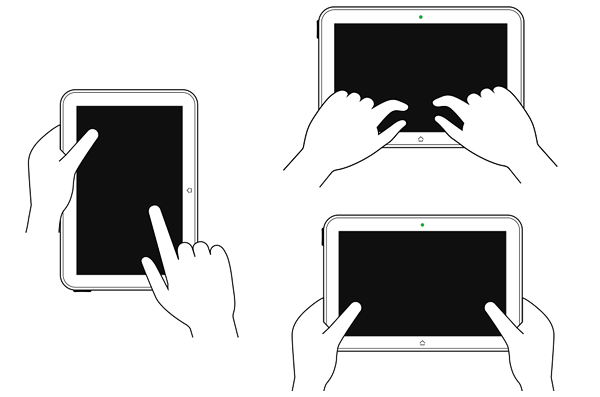
\includegraphics[width=\textwidth]{img/tnav-touch-tablets.png}
        \end{subfigure}%
         %add desired spacing between images, e. g. ~, \quad, \qquad etc.
          %(or a blank line to force the subfigure onto a new line)
        \begin{subfigure}[b]{0.4\textwidth}
                \centering
                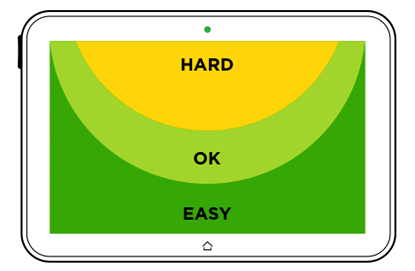
\includegraphics[width=\textwidth]{img/tnav-touch-tablets2.png}
        \end{subfigure}

        \caption[Schopnosť ovládania tabletov]{Schopnosť ovládania tabletov \cite{navigation}.\\
		Prevzaté z http://www.lukew.com/ff/entry.asp?1649}
		\label{fig:tnavtablets2}
\end{figure}

Podobné výsledky \cite{mobilebooktouch} sú aj pri novej kategórii zariadení, tzv. hybridných notebookov, ktoré okrem klávesnice obsahujú aj dotykový displej.

\begin{figure}[H]
	\centering
	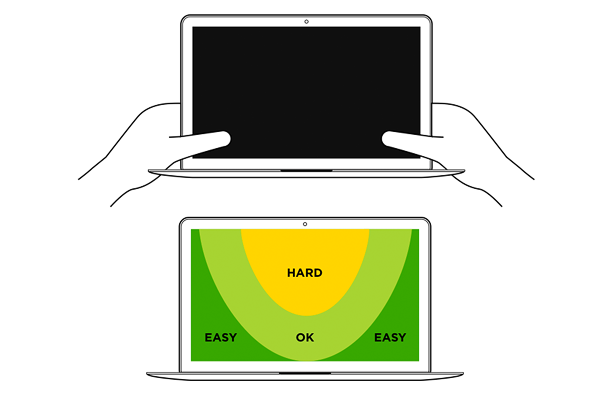
\includegraphics[width=0.5\textwidth]{img/tnav-touch-laptops.png}
	\caption[Schopnosť ovládania hybridných počítačov]{
		Schopnosť ovládania hybridných počítačov \cite{navigation}.\\
		Prevzaté z http://www.lukew.com/ff/entry.asp?1649}
	\label{fig: tnavlaptops}
\end{figure}

Najlepší interfejs na ovládanie webu je však niekedy úplne bezdotykový. Môžeme použiť ďalšie senzory a rečový vstup, ktorý je ďalším zlepšením interakčného dizajnu.

\paragraph{Reč} % (fold)

Ovládanie aplikácii a zariadení pomocou reči môže byť užitočné pre prípady spojené s indispozíciou používateľov najmä v spojení so slabším zrakom či fyzickým postihnutím \cite{SpeechRecognition}.

Možnosť rozpoznania reči vo webovej aplikácii je v súčasnosti experimentálna novinka a jej štandardizácia je zatiaľ veľmi ďaleko. Používateľ samozrejme musí explicitne povoliť použitie mikrofónu pre webovú aplikáciu. Špecifikácia je zatiaľ len vo forme návrhu a nie je ani zaradená do W3C štandardu HTML5 \cite{webspeechapi}. Podpora v prehliadočoch s enginom Blink sa však už nachádza od začiatku roku 2013 a základná funkčnosť bola odprezentovaná v rámci konferencie Google IO 2013. Rozpoznanie reči prebieha vzdialene na serveroch patriacich Googlu a zatiaľ neexistuje možnosť rozpoznania lokálne \cite{moreawesomeweb}.

S rozpoznaním reči je spojená aj jeho syntéza, alebo preklad textu na reč. Tá je na tom v súčasnosti čo sa týka podpory a implementácie v prehliadačoch ešte horšie. Experimentálna funkčnosť existuje len v posledných buildoch prehliadočov. Našťastie sa táto funkcionala dá čiastočne nahradiť volaniami vzdialených webových služieb ako je napríklad ,,Google Translate''. Takáto syntéza však už neprebieha na zariadení, ale len sa zo serveru príjme zvuková nahrávka, ktorá sa následne prehrá.

\newpage
\paragraph{Pohyb používateľa} % (fold)

Rozpoznanie pohybu v reálnom čase je možné určiť podľa udalostí uskutočnených používateľom. Jednou z možností je použiť algoritmus na základe zmeny osvetlenia objektu \cite{MotionIllumination} a tým určiť smer jeho pohybu.

Moderné webové prehliadače umožňujú získať prístup aj k video streamu z web kamery používateľa. Na prístup je rovnako potrebné povolenie od používateľa. Tento video stream prebieha vo zvolenej frekvencii a sa dá odchytiť a následne uložiť do elementu canvas, kde už sa k jednotlivým vzorkám pristupuje ako k obrázku. Je možné odfiltrovať okolie a zachovať len podstatné informácie na základe ktorých sa získa pohyb, respektíve gesto od používateľa.


\paragraph{Pohyb zariadenia} % (fold)

Na detekovanie pohybu zariadenia môžme použiť množstvo senzorov. Jednou z možností je použitie kombinácie vždy snímajúcich senzorov ako sú accelerometer, gyroskop a magnetometer, ktoré nám povedia ako sa zariadenie pohybuje v priestore. Schopnosť použitia týchto senzorov na poskytnutie presných informácií o pohybe zariadenia nám prináša množstvo nových možností v dizajne webových aplikácii \cite{ultrabooks}.

Medzi dlhodobo podporované senzory najmä v mobilných zariadeniach patria accelerometer a gyroskop. Je k nim umožnený prístup priamo z webovej aplikácie aj bez priameho povolenia od používateľa. Dáta z nich získané je zároveň možné použiť na vytvorenie a rozpoznanie giest použitých na ovládanie aplikácie \cite{AccelerationAndGyroscope}.

Accelerometer slúží na získanie zrýchlenia zariadenia v osiach x, y a z, gyroskop na získanie uhlového zrýchlenia okolo týchto osí. Ich rozdiel je znázornený na nasledujúcom obrázku:

\begin{figure}[H]
  \centering
  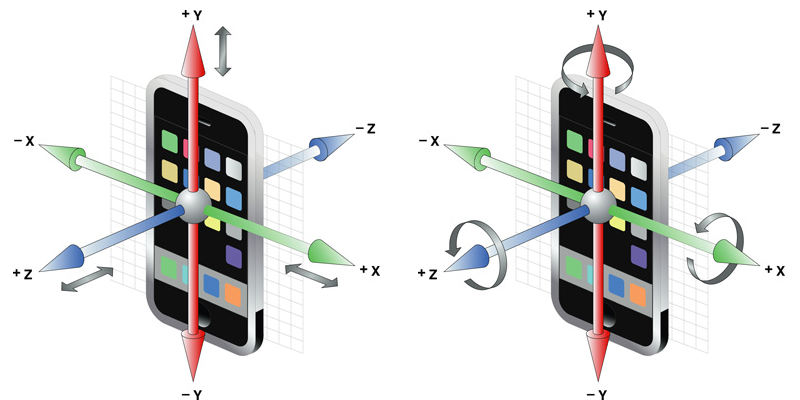
\includegraphics[width=0.8\textwidth]{img/accvsgyro.png}
  \caption[Accelerometor a gyroskop]{
    Zaznamenávané údaje pomocou accelerometora a gyroskopu}
  \label{fig: tnavlaptops}
\end{figure}

% subsubsection interak_n_prostriedky (end)

\newpage
\subsubsection{Pripojenie} % (fold)
\label{ssub:pripojenie}

Spoločnou vlastnosťou webových aplikácii je, že pristupujú k rôznym zdrojom, ktoré sa môžu nachádzať okrem lokálneho úložiska aj na serverom, pomocou internetu. Spôsoby prenosu dát sú rôzne, od pevného pripojenie cez bezdrôtové až po mobilné, a každé z nich má iné vlastnosti.

V poslednom období sa spolu s mobilnými zariadeniami rozširuje aj používanie mobilného internetu. Keďže našim cieľom je, aby sa webová stránka načítala používateľovi čo najrýchlejšie, respektíve ak chceme aby sa používateľ na našu stránku prišiel a príchod si nerozmyslel pri jej dlhom načítavní, tak musíme šetriť množstvom prenášaných dát. Takéto šetrenie dát zároveň šetrí aj peňaženky používateľov \cite{performance}, hlavne pokiaľ sa jedná o roamingové dáta v zahraničí.

Načítanie webovej stránky sa skladá z viacerých fáz. Okrem samotnej konektivity používateľa aj spracovanie požiadavky serverom a následne vykonanie akcie v prehliadači. To je jediná fáza, ktorú môžeme ovplyvniť.

\begin{figure}[H]
	\centering
	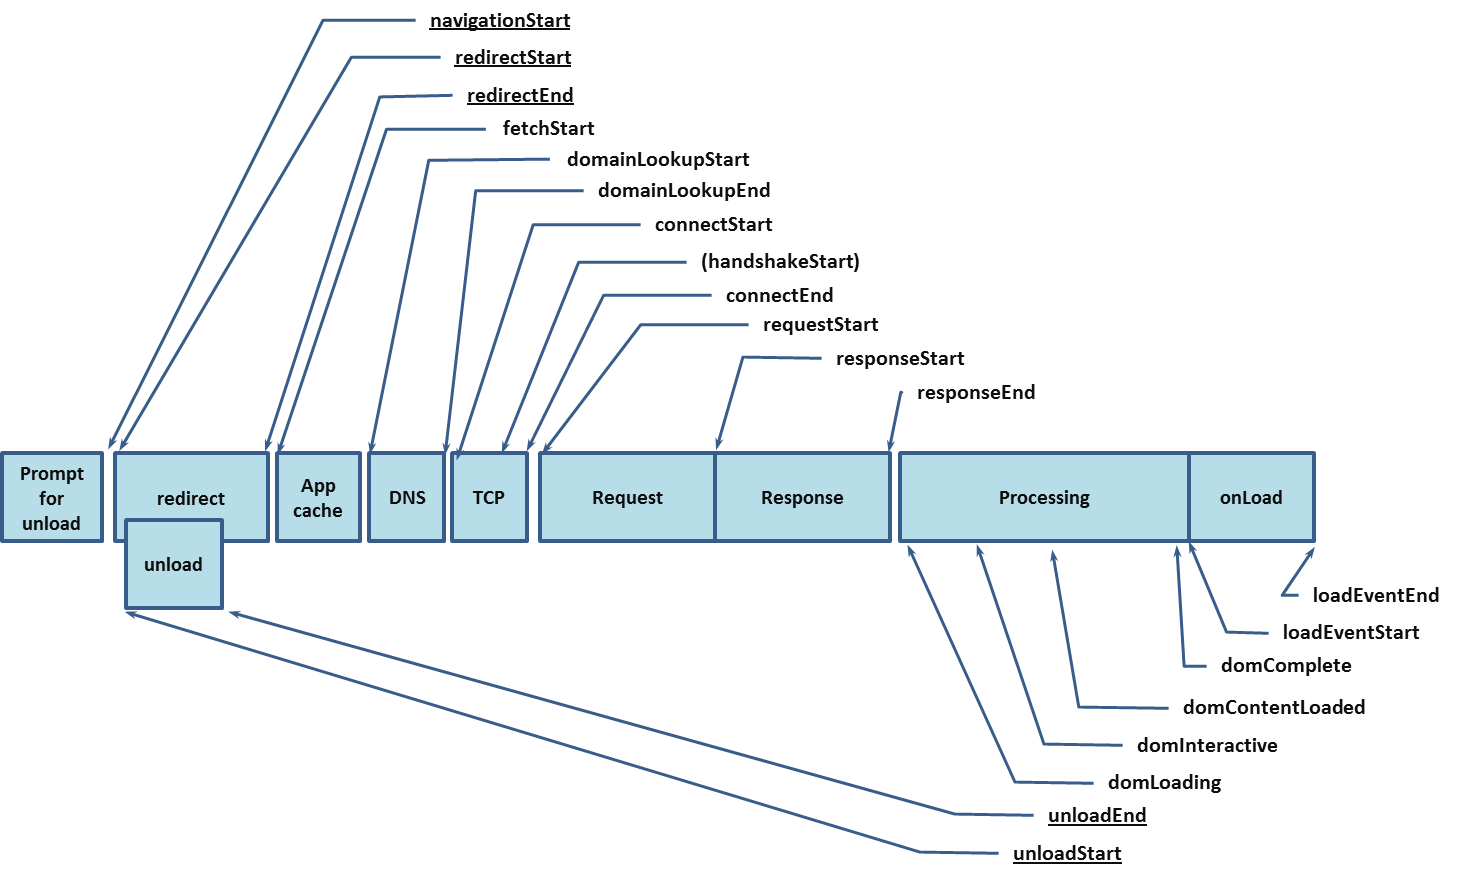
\includegraphics[width=0.9\textwidth]{img/w3c-timing-overview.png}
	\caption[Fázy spracovania požiadavky na server]{
		Fázy spracovania požiadavky na server \cite{timing}.\\
		Prevzaté z http://www.w3.org/TR/navigation-timing/}
	\label{fig: timing}
\end{figure}

Tieto fázy môžme aj priamo merať pomocou interfacu \url{performance.timing}, ktorý ich zobrazuje priamo v podobe času \cite{1000ms, performancebrowsernetworking}. Vďaka tomu máme dokonalejší prehľad o používateľovom pripojení a vieme mu tak prispôsobiť jednotlivé komponenty stránky. W3C špecifikácia je vo fáze ,,Recommendation'' \cite{timing}, ale stále hlavnou nevýhodou je chýbajúca podpora v niektorých prehliadačoch. Čiastočnou náhradou je meranie rozdielov dvoch časov, ale tak získame dáta len zo spracovania požiadavky na strane klienta.

\begin{figure}[H]
	\centering
	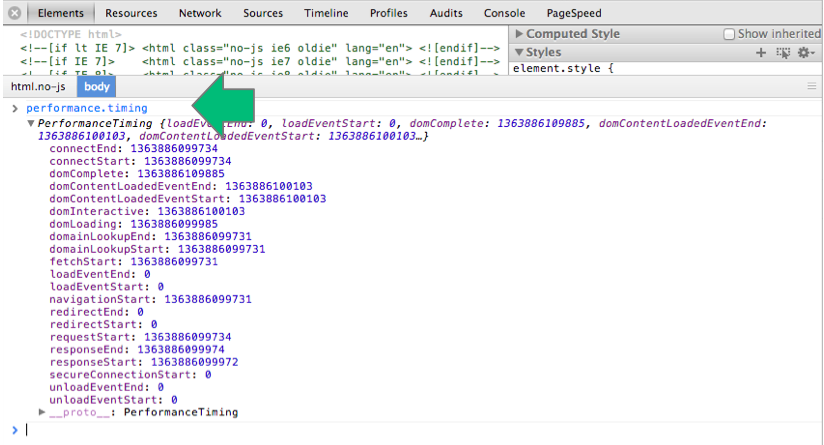
\includegraphics[width=0.9\textwidth]{img/1000ms.png}
	\caption[Čas potrebný na spracovanie požiadavky na server]{
		Čas potrebný na spracovanie požiadavky na server.}
	\label{fig: 1000ms}
\end{figure}

Každá požiadavka na server niečo stojí. Ideálny prípad je taký, že medzi zariadením a serverom sa neprenášajú žiadne dáta a všetky prístupy ku zdrojom sa riešia len z lokálneho úložiska. V prípade internetových aplikácii to však väčšinou nie je úplne možné, pretože používateľ chce pristupovať k čo najčerstvejším dátam. Cieľom je však čo najviac limitovať požiadavky na server.

To, či je vôbec používateľ pripojený na internet vieme zistiť pomocou interfacu \url{navigator.onLine}, ktorý vráti hodnotu ,,true'' alebo ,,false'' a takisto môžme počúvať na zmeny pripojenia vďaka ,,event listenerom'' na \url{window.online} a \url{window.offline}.

Rýchlosť, akou je používateľ pripojený na internet, je dostupná v objekte \url{navigator.connection} pod atribútom ,,bandwidth'' charakterizujúcej pripojenie v MB/s \cite{network}. V prípade zmeny rýchlosti je rovnako vyvolaný ,,event''. Nevýhodou je zatiaľ slabá podpora zo strany prehliadačov.

% subsubsection pripojenie (end)

\subsubsection{Platforma} % (fold)
\label{ssub:platforma}

Rozhodovanie sa na základe platformy je taktiež veľmi dôležité. Umožňuje nám jednak zjednošiť dizajn a zmenšiť počet potrebných komponentov na webovej stránke, ale taktiež vytvárať cielenú reklamu. Rozlišovanie prebieha na základe pola ,,user agent'' špecifickom pre každý prehliadač, respektíve operačný systém.

V prípade zisťovania podpory jednotlivých vlastností je však lepšie priamo zisťovať podporu komponentu zo strany prehliadača ako zisťovaním a porovnaním s platformou. Nemusíme si tak udržiavať databázu a neustále ju aktualizovať. Takéto riešenie je preto z pohľadu vývoja lepšie pre budúcnosť.

% subsubsection platforma (end)

% subsection mo_nosti_prisp_sobenia (end)

\newpage

\subsection{Adaptačné techniky \footnote{Tejto kapitole som sa už z časti venoval vo svojej bakalárskej práci Tvorba bohatých internetových aplikácií pre mobilné zariadenia \cite{ja}. V tomto dokumente sa nachádza rozšírená verzia doplnená o novo vzniknuté techniky adaptácie.}} % (fold)
\label{sub:adapta_n_techniky}

S príchodom prvých mobilných zariadení existoval rozdiel medzi mobilným webom a webom pre desktopy a tak bolo pomocou servera jednoduché zistiť, aká verzia sa má zariadeniu zobraziť.

Pretože dnes už existuje mnoho zariadení od mobilných cez tablety až po klasické počítače a vzájomne sa prelínajú, je potrebné zabezpečiť, aby sa webový obsah zobrazoval správne na každom z nich.\\

\begin{fancybox}
\textit{,,There is no Mobile Web. There is only The Web, which we view in different ways. There is also no Desktop Web. Or Tablet Web. Thank you.'' Stephen Hay} \cite{noMobileWeb}
\end{fancybox}

Tento výrok bol vyslovený už pred niekoľkými rokmi a v súčasnosti pri prelínaní rôznych zariadení sa stále viac potvrdzuje. Pre vývoj webovej stránky alebo aplikácie existuje viacero spôsobov \cite{mobiforge}, každý má svoje výhody a nevýhody. Správnosť výberu konkrétnej metódy záleži od toho, či ideme upravovať už existujúcu webovú verziu na rôzne zariadenia alebo či vytvárame novú aplikáciu a v neposlednom rade aj od vynaloženého úsilia či financií.


\subsubsection{Responsive design} % (fold)
\label{ssub:responsive_design}

Pojem ,,Responsive design'' pôvodne zahŕňal pravidlá tvorby dizajnu pre rôzne rozlíšenia a bol špecifikovaný v roku 2010. Všetkým zariadeniam sa posiela rovnaký HTML a javascript, rozdiel je len v dizajne. Dizajn sa zakladá na používaní flexibelného vzhľadu stránky, ktorý sa prispôsoboval rôznym zariadeniam, flexibilných obrázkoch, ktorých veľkosti sa prispôsobujú vzhľadu a CSS media queries. \cite{responsive, mediaqueries} Až neskôr bol označený ako metóda na dosiahnutie výsledku.

Tvorba vzhľadu pomocou Responsive design znamená aplikáciu rozmerov jednotlivých elementov v percentuálnom pomere namiesto statických hodnôt, ktoré sa tak automaticky prispôsobujú rôznym veľkostiam. Ďalej sa vytvára webová stránka pre referenčné rozlíšenie a pomocou CSS media queries sa pridávajú ďalšie pravidlá pre elementy ako by mali vyzerať pri iných rozlíšeniach, orientácii či pomere strán. Pri použití takéhoto prístupu však nastávajú problémy správnosti zobrazenia na zariadeniach s menším či väčším rozlíšením displeja vzhľadom k ich fyzickej veľkosti, napríklad keď má televízor menšie rozlíšenie ako mobilné zariadenie.


\paragraph{Výhody:}
\begin{itemize}
	\item dosiahnutie nezávislosti zobrazenia pri rôznom rozlíšení zariadení, umožňuje prispôsobiť stránky pre mobilné zariadenia, tablety či stolové počítače
	\item umožňuje rýchlu tvorbu aplikácie
\end{itemize}

\paragraph{Nevýhody:}
\begin{itemize}
	\item neumožňuje prispôsebenie obsahu, ale len jeho zobrazenie, sťahujú sa všetky zdroje
	\item problémy pri zariadeniach s nepomerným rozlíšením displeja vzhľadom k fyzickej veľkosti
\end{itemize}

% subsubsection responsive_design (end)


\subsubsection{Mobile First} % (fold)
\label{ssub:mobile_first_responsive_design}

Postupný rozmach mobilných zariadení s menšími rozlíšeniami a veľkosťami displejov podnietil vznik novej metódy dizajnu - ,,Mobile First''. Základ tvorí metóda Responsive design, ale pôvodný návrh stránky sa nerobí pre desktopovú verziu ale na malé rozlíšenie mobilného zariadenia. Až pomocou media queries sa postupne prispôsobujú pravidlá elementov pre väčšie a väčšie rozlíšenie. Takto sa webová stránka prispôsobí pre všetky rozlíšenia od najmänších až po tie najväčšie a zároveň je pripravená aj na ešte neexistujúce zariadenia, ktoré budú mať oveľa väčšie rozlíšenie ako majú tie súčasné.

Technika Mobile First však okrem samotného prispôsobenia zobrazenia stránok zahŕňa aj optimalizáciu webu pre používateľa či už z pohľadu UX alebo výkonu \cite{mobilefirst}. Predpokladá, že používateľ na web pristupuje najmä z mobilného zariadenia a tak sa mu snaží čo najviač tento pobyt spríjemniť. Minimalizuje sa množstvo údajov potrebných pre vyplnenie formulárov alebo sa pripraví zobrazenie správnej klávesnice pre zadávanie číselných vstupov, emailov či čistého textu bez toho, aby ju sám musel prepínať.

\paragraph{Výhody:}
\begin{itemize}
	\item umožňuje zobrazeniť obsah pre rôzne rozlíšenia zariadení
	\item pokrýva zariadenia od najmenších až po tie najväčšie a zároveň webová stránka je pripravená aj na ,,zariadenia budúcnosti''
  \item vylepšenie UX
\end{itemize}

\paragraph{Nevýhody:}
\begin{itemize}
	\item neumožňuje prispôsebenie obsahu, ale len úpravu vzhľadu
	\item pri existencii súčasneho riešenia webu sa dizajn stránky musí vytvorať od základu, čo však môže byť aj východa
\end{itemize}

% subsubsection mobile_first_responsive_design (end)

\subsubsection{Progressive enhancement} % (fold)
\label{ssub:progressive_enhancement}

S nástupom HTML5 sa v poslednom období sa stáva veľmi popolárnou metódou Progressive Enhancement. Táto metóda je založená na princípe posielania jednotného počiatočného zdrojového kódu všetkým zariadeniam a umožňuje vytvoriť takzvanú ,,single page application''. Vykonávanie logiky aplikácie sa úplne presúva zo strany servera na klienta kde prebieha pomocou javascriptu. Tam sa ďalej presne špecifikuje čo, kedy a ako sa má vykonávať. 

Každému zariadeniu je umožnený základný prístup k webu a jeho obsahu. Pokiaľ však zariadenie, respektíve použítý webový prehliadač, podporuje pokročilejšie vlastnosti potrebné na beh aplikácie či prístup k senzorom, tak je mu ponúknotá obohatená verzia. Taktiež je možné doťahovať ďalšie zdroje zo servera len vtedy keď sú potrebné a tým sa zabraňuje zbytočným prenosom dát. Pomocou využívania pokričelejších možností HTML5 je dokonca možné tvoriť offline klientské webové aplikácie.

Pokiaľ chceme pokryť celé spektrum zariadení tak je implementácia pomocou tejto metódy náročnejšia. V spojení s metódou reseponsive design je to ale výborné riešenie na prispôsobenie si obsahu a vzhľadu aplikácie.

\paragraph{Výhody:}
\begin{itemize}
	\item úplne prispôsobenie obsahu a vzhľadu
  \item minimálne alebo žiadne dátove prenosy
\end{itemize}

\paragraph{Nevýhody:}
\begin{itemize}
	\item náročnejšia implementácia, 
	\item rýchlosť vykonávania aplikácie závisi od výkonu zariadenia
\end{itemize}

% subsubsection progressive_enhancement (end)

\subsubsection{Graceful degradation} % (fold)
\label{ssub:graceful_degradation}

Vykonávanie aplikácie prebieha na zariadení, je však opačné ako v prípade metódy Progressive enhancement. Používateľovi sa predáva plne funkčná aplikácia nadizajnovaná na najlepšie zariadenia, kde sa na jednotlivé pokročilejšie funkcie postupne vypínajú ak nie sú dostupné pre použité zariadenie. Používa sa často na upravenie súčasnej už nasadenej verzie na potreby mobilných zariadení.

\begin{figure}[H]
	\centering
	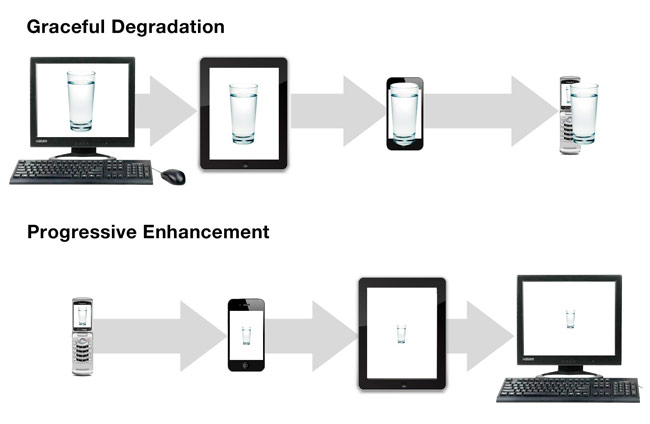
\includegraphics[width=0.8\textwidth]{img/PEvsGD.jpg}
	\caption[Progressive enhancement vs Graceful degradation]{
		Progressive enhancement vs Graceful degradation \cite{adaptivesxsw}.\\
		Prevzaté z http://bradfrostweb.com/blog/web/mobile-first-responsive-web-design/}
	\label{fig: gd}
\end{figure}

\paragraph{Výhody:}
\begin{itemize}
	\item prispôsobenie obsahu a vzhľadu na jednoducšie zariadenia
	\item zachovanie súčasnej verzie webovej stránky
\end{itemize}

\paragraph{Nevýhody:}
\begin{itemize}
	\item nezohľadňuje budúce zariadenia, už v súčasnosti majú niektoré tablety kvalitnejšie displeje ako stolové počítače 
\end{itemize}

% subsubsection graceful_degradation (end)


\subsubsection{Server-side Adaptation} % (fold)
\label{ssub:ress_}

Metóda Server-side Adaptation je používaná väčšinou webových stránok na detekovanie mobilného zariadenia a v súčasnosti patrí už medzi historické techniky. Pri prístupe na stránku sa pomocou servera detekuje zariadenie a je mu ponuknutá vhodná verzia stránky, väčšinou dochádza k presmerovaniu (na mobilnú verziu). Celá logika aplikácie sa nachádza na serveri. Stránka môže byť presne vytvorená pre dané zariadenie, takže nenastávajú problémy pri dizajne, je však potrebné mať na serveri nainštalovanú knižnicu na jeho detekovanie\footnote{napríklad DeviceAtlas alebo WURFL založené na detekovaní pola user agent}. Detekcia zariadenia je pri priamej návšteve stránky cez prehliadač úspešná, k problémom však prichádza pri návšteve stránky cez iných klientov. Taktiež je dôležité mať databázu zariadení neustále aktualizovanú.

\paragraph{Výhody:}
\begin{itemize}
	\item zobrazenie vhodnej stránky pre zariadenie, nesťahuje sa nepotrebný obsah
\end{itemize}

\paragraph{Nevýhody:}
\begin{itemize}
	\item potreba knižníc na detekovanie zariadenia, ktorú je nutnú neustále aktualizovať
	\item dlhšie načítavanie stránky na pomalšom internetovom pripojení, pretože dochádza k presmerovaniu
\end{itemize}

V súčasnosti sa táto metóda nahrádza pomocou metódy RESS alebo Progressive enhancement. Stále však potrebujeme informácie o type zariadenia a tak vznikajú mnohé knižnice ako napríklad WURFL.js\footnote{\url{http://wurfl.io/}} ktoré nám informácie o ňom prezradia aj na strane klienta.

% subsubsection ress_ (end)

\subsubsection{RESS (Responsive Design + Server Side Components)} % (fold)
\label{ssub:ress_responsive_design_server_side_components_}

Kombináciou techník Responsive Design a Server-side Adaptation vznikla novšia technika adaptácie. Pre každý typ zariadenia sa na serveri dynamicky vygenerujú pre neho špecifické komponenty webovej aplikácie, ktoré sa mu následne zobrazia a upravia sa na strane klienta pomocou responsive dizajnu. Pomocou detekcie zariadenia sa však určí či sa samotný komponent má do výsledku pridať, respektíve či sa má nahradiť nejakým iným.

\paragraph{Výhody:}
\begin{itemize}
	\item jednoduchšia udržiaveteľnosť, neexistujú rôzne verzie stránky ale len jedna z viacerými komponentami
\end{itemize}

\paragraph{Nevýhody:}
\begin{itemize}
	\item potreba nainštalovaných knižníc na detekovanie zariadenia
	\item náročnejšia implementácia na strane servera
\end{itemize}

% subsubsection ress_responsive_design_server_side_components_ (end)

% subsection adapt_cia (end)

\newpage
\section{Návrh riešenia} % (fold)
\label{sec:n_stroj_na_overenie}

V tejto časti práce sa venujem návrhu jednotlivých súčastí systému, ktoré umožnia adaptáciu webovej aplikácie na rôzne zariadenia. Vytvorenie jednotlivých súčastí knižnice vzišlo z potrieb komunity vývojárov a samotného trhu. Skúmali sa najmä možnosti alternatívnych spôsobov ovládania aplikácie a adaptácia používaných komponentov. Alternatívne možnosti ovládania aplikácii sú veľmi populárne a v prostredí webových aplikácií chýbal nástroj, ktorý by umožnil jednoduchú interakciu používateľa s aplikáciou. Potrebné bolo riešiť aj veľké množstvo zbytočne prenášaných dát pomocou internetu v prostrediach a na zariadeniach, ktoré ich všetky nepotrebujú.

Ako nástroj na overenie adaptácie sa vytvorila knižnica s názvom Angular-Adaptive\footnote{Vytvorená knižnica Angular-Adaptive \url{http://angular-adaptive.github.io/} je pomocník vo svete adaptívneho web dizajnu.} do populárneho JavaScriptového frameworku AngularJS, kde sa následne skúmali možnosti adaptácie komponentov pomocou metódy progressive enhancement.

Hlavným dôvodom výberu AngularJS bola možnosť vytvárania modulov, ktoré sa dajú následne jednoducho použivať vo webových projektoch. Takáto podpora vytvárania externých modulov bude už o pár rokov natívna v prehliadačoch vďaka webovým komponentom \cite{webcomponents}. Samotná distribúcia modulov prebieha pomocou balíčkovaciemu nástroja Bower\footnote{Bower \url{http://bower.io/} je balíčkovací manažér pre web.}, ktorý je v súčasnosti štandardným distibučným miestom webových komponentov.

\begin{figure}[H]
  \centering
  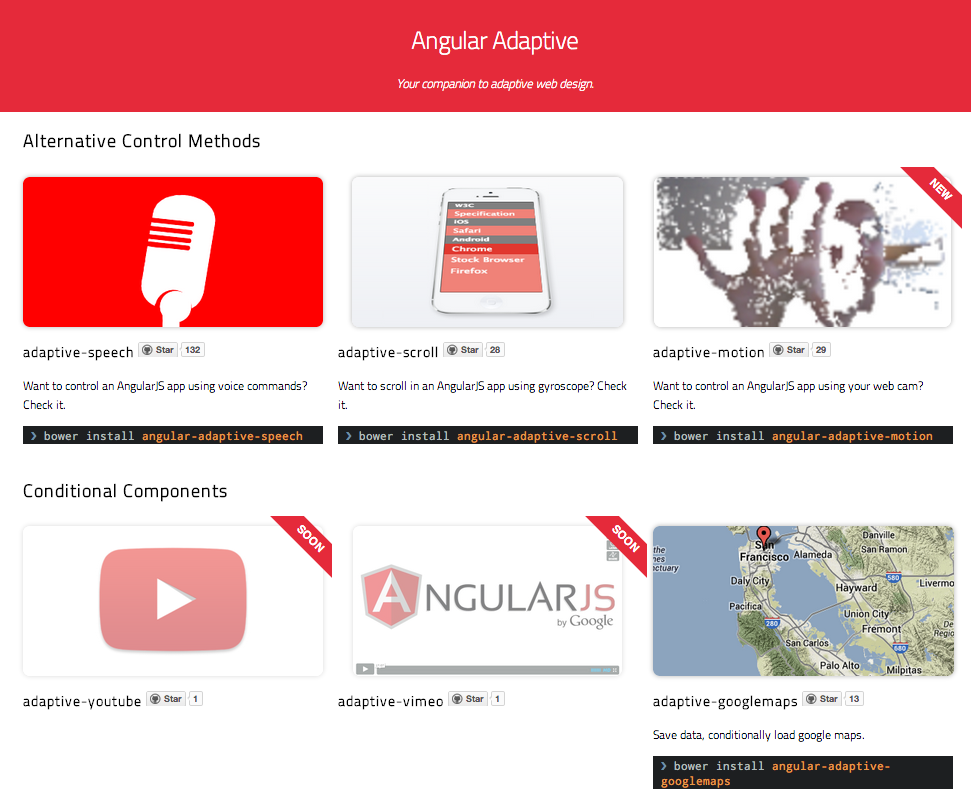
\includegraphics[width=0.7\textwidth]{img/angularadaptive.png}
  \caption[Webová stránka vytvoreného projektu angular-adaptive]{
    Webová stránka vytvoreného projektu angular-adaptive}
  \label{fig: angularadaptive}
\end{figure}

\newpage
Celý systém je možné rozdeliť do troch na sebe navzájom nezávislých logických celkov skladajúcich sa z nasledujúcich častí:

\begin{enumerate}
  \item alternatívne spôsoby ovládania webovej apliekácie, kde sa vytvorili knižnice na ovládanie pomocou reči, pohybu a gyroskopu
  \item adaptácie webových komponentov použitých v aplikáciách, kde sa skúmali hlavne ich možnosti prispôsobenia sa jednotlivým zariadeniam a internetovému pripojeniu používateľa
  \item nástroje použité na implementáciu aplikácie
\end{enumerate}

V nasledujúcich častiach kapitoly opisujem návrh implementácie jednotlivých súčastí systému.

\subsection{Alternatívne spôsoby ovládania} % (fold)
\label{sub:alternat_vne_sp_soby_ovl_dania}

Príchod mobilných zariadení priniesol a spopularizoval nový spôsob interakcie - ovládanie zariadenia pomocou dotyku. Ten však vždy nemusí byť ten najvýhodnejší najmä v prostredí webových aplikácií. Súčasné moderné zariadenia obsahujú množstvo senzorov. Najmä mobilné zariadenia sú vybavené gyroskopom, ktorý môže uľahčiť ovládanie aplikácie len vďaka nakláňaniu zariadenia do strán. Podobne môže reagovať zariadenie sledovaním okolia vďaka vstupu z webovej kamery, ktorá je vstavaná v množstve zariadení. Typickým senzorom v zariadeniach je mikrofón umožňujúci zaznamenať zvuk, z ktorého sa analyzujú rečové povely a tie vedia zefektívniť ovládanie aplikácie.

\subsubsection{Reč} % (fold)
\label{ssub:re_}

Ovládanie mobilných zariadení pomocou rečových povelov sa v posledných rokoch teší narastajúcej popularite. Rozpoznávanie je ale špecifické pre jednotlivé mobilné platformy. Javascriptové Web Speech API však umožňuje pridanie rozpoznania reči aj do webovej aplikácie. 

Cieľom je umožniť ovládanie aplikácie zadávaním statických povelov, ale aj ovládať dynamicky vytvárané entity v aplikácii nezávislé od zvoleného jazyka používateľa. Ovládanie aplikácie by malo prebiehať kontinuálne bez akejkoľvek ďalšej potrebnej interakcie používateľa. Na ich základe bol vytvorený modul ktorý umožňuje pridať kompletné ovládanie webovej aplikácie. Používateľ všal musí povoliť prístup aplikácie k mikrofónu. Po jeho potvrdení už prebieha kontinuálne rozpoznávanie reči.

Po pridaní modulu do webovej aplikácie je potrebné si ho nakonfigurovať. Musia sa vytvoriť úlohy, ktoré definujú správanie aplikácie a prípadne aj reč, v ktorej prebieha rozpoznávanie. Implementované rozpoznávanie reči v prehliadači Google Chrome podporuje 32 rôznych jazykov a ďalšie prízvuky vrátane slovenčiny.

Rozpoznanie úloh prebieha na základe regulárneho výrazu definovaného v konfigurácii danej úlohy. Vďaka tomu je zaručené, že ako rozpoznaný text sa získa dynamicky reťazec s ktorým je možné ďalej v aplikácii pracovať. 

Nakoľko je v aplikácii dôležitá viacjazyčná podpora je potrebné ju správne definovať rozlíšením kódu jazyka úlohy. Keď sa aktuálne nastavený jazyk rozpoznávania zhoduje s jazykom v úlohe a rozpoznaný text spĺňa podmienku regulárneho výrazu, tak sa zavolá asociovaná callback funkcia. Tá v parametri obsahuje rozpoznaný text v podobe textového reťazca, s ktorým sa dá ďalej pracovať. Príklad konfigurácie na pridanie novej úlohy má nasledujúci tvar:

\begin{lstlisting}
'someTask': {
  'regex': /^do .+/gi,
  'lang': 'en-US',
  'call': function(utterance){
    // do something with utterance
  }
}
\end{lstlisting}


Takýchto konfigurácií je možné pridať ľubovoľný počet. Takto navrhnutú konfiguráciu je možné zavolať globálne v rámci aplikácie alebo dynamicky vďaka podpore regulárneho výrazu a frameworku AngularJS pre dynamicky vytvárané elementy. V prípade globálneho volania stačí použiť samotnú konfiguráciu:

\begin{lstlisting}
$speechRecognition.listenUtterance(
  $scope.recognition['en-US']['someTask']
);
\end{lstlisting}

Pri dynamicky vytváraných elementoch je okrem samotnej konfigurácie s regulárnym výrazom potrebné pridať aj vstupný prvok elementu voči ktorému sa bude rozpoznávanie vykonávať. Takto sa vzájomne rozlíšia jednotlivé dynamické elementy a asociovaná úloha sa vykoná len pre jeden prvok.

\begin{lstlisting}
$scope.todos = ['buy milk', 'write essay'];

<li ng-repeat="todo in todos">
  <div speechrecognition="{'tasks': recognition['en-US']['someTask'], 'input': todo}">{{todo}}</div>
</li>
\end{lstlisting}

Napríklad ak sa v aplikácii pracuje so zoznamom úloh, tak globálne je možné obsluhovať pridanie novej úlohy a dynamicky vytvárané elementy môžu mať vlastnú obsluhu, ktorá počúva na ich meno. 

Niekedy je potrebné v aplikácii na istý čas ignorovať ovládanie pomocou reči. Kvôli takýmto prípadom sa pridala možnosť jeho nastavenia v podobe metódy payAttention. Diagram navrhnutého algoritmu ovládania webovej aplikácie pomoc reči sa nachádza na nasledujúcom obrázku:

\begin{figure}[H]
  \centering
  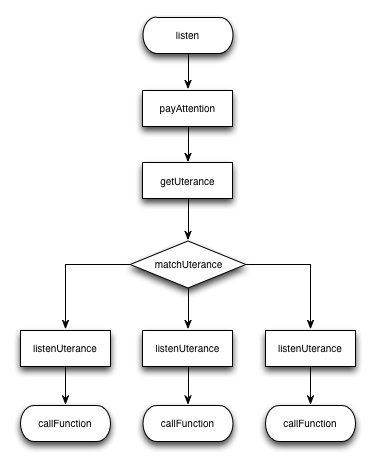
\includegraphics[width=0.75\textwidth]{diagram/speech.png}
  \caption[Algoritmus ovládania aplikácie pomocou reči]{
    Algoritmus ovládania aplikácie pomocou reči}
  \label{fig: diaspeech}
\end{figure}

Použitie regulárneho výrazu pri konfigurácii úlohy má samozrejme aj nevýhodu. Najväčšou je potrebnosť presného určenia výrazu, nakoľko v opačnom prípade sa môžu detekovať aj nesprávne príkazy. Nevyhnutnosťou je aj stále pripojenie na internet kvôli vzdialenému rozpoznaniu reči, pričom samotné rozpoznanie nemusí byť vždy správne.

% subsubsection re_ (end)

\subsubsection{Pohyb} % (fold)
\label{ssub:pohyb}

Ovládanie webovej aplikácie pohybom prebieha vďaka webovej kamere. Cieľom riešenia je rozpoznať základné smery pohybov používateľa a umožniť na ne namapovať funkcionalitu aplikácie, ktorá sa vykoná po ich správnom rozpoznaní. 

Video sa sníma kontinuálne a zachytený video stream z kamery je s frekvenciou 60 fps. Každý jeden snímok je následne vykreslený do elementu canvas, v ktorom je možné s ním pracovať. Ten je tvorený množinou pixelov s rgba hodnotami.

\begin{figure}[H]
  \centering
  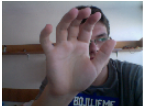
\includegraphics[width=0.3\textwidth]{img/motion/video.png}
  \caption[Vizualizácia videa zachyteného web kamerou]{
    Vizualizácia videa zachyteného web kamerou}
  \label{fig: motion-video}
\end{figure}

Získaný obrázok sa následne upraví pomocou hsv filtra aplikovaného na všetky pixely aby sa detekovali oblasti s kožou používateľa, pričom hsv filter je možné nakonfigurovať na vlastné hodnoty. Vďaka týmto oblastiam je rozpoznaný používateľ a je možné spracovávať jednotlivé smery pohybov. Upravený snímok je tvorený dvomi farbami: tmavou znamenajúcou kožu a bielou pre ostatné oblasti. Rozpoznanie prebieha nasledovne:

\begin{lstlisting}
if ( (
    (hsv[0] > hsvFilter.huemin && hsv[0] < hsvFilter.huemax) || 
    (hsv[0] > hsvFilter.losemin && hsv[0] < losemax)
  ) && 
  (hsv[1] > hsvFilter.satmin && hsv[1] < hsvFilter.satmax) &&
  (hsv[2] > hsvFilter.valmin && hsv[2] < hsvFilter.valmax)
) {
  skinFilter[pix] = r;
  skinFilter[pix+1] = g;
  skinFilter[pix+2] = b;
  skinFilter[pix+3] = a;
}
\end{lstlisting}

\begin{figure}[H]
  \centering
  
\includegraphics[width=0.3\textwidth]{img/motion/skin.png}
  \caption[Vizualizácia videa po aplikovaní filtra detekcie kože]{
    Vizualizácia videa po aplikovaní filtra detekcie kože}
  \label{fig: motion-skin}
\end{figure}

Ako je možné vidieť, detekcia kože nie je úplne správna a na základe hsv sa detekuju aj iné oblasti. Následne prebieha ďalšie upravovanie pri ktorom sa detekuju len samotné hrany. Ich detekcia prebieha na základe rozdielov farebnosti pixelov posledných dvoch snímkov \cite{MotionIllumination} s aplikovaným filtrom kože. Zistí sa celkový rozdiel v rgba hodnote každého pixelu a pokiaľ nastala výrazná zmena, tak sa detekuje ako hrana a zafarbí sa:

\begin{lstlisting}
var rgbaDelta = Math.abs(draw.data[pix] - lastDraw.data[pix]) +
  Math.abs(draw.data[pix+1] - lastDraw.data[pix+1]) +
  Math.abs(draw.data[pix+2] - lastDraw.data[pix+2]);

if (rgbaDelta > treshold.rgb){
  edge.data[pix] = 0;
  edge.data[pix+1] = 0;
  edge.data[pix+2] = 0;
  edge.data[pix+3] = 255;
}
\end{lstlisting}

Opäť vznikne snímok tvorený dvomi farbami, ale tentokrát tmavá farba sa nachádza len na hranách a biela na ostatných častiach obrázku. Obrázok definuje miesta, na ktorých sa medzi snímkami vykonával pohyb. Na základe sekvencie takýchto obrázkov hrán vieme presnejšie určiť smer pohybu používateľa.

\begin{figure}[H]
  \centering
  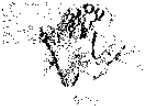
\includegraphics[width=0.3\textwidth]{img/motion/edges.png}
  \caption[Vizualizácia videa po aplikovaní filtra detekcie hrán]{
    Vizualizácia videa po aplikovaní filtra detekcie hrán}
  \label{fig: motion-edges}
\end{figure}

Keď je obrázok v už takomto stave tak je možné začať rozpoznávať predvádzané gesto. Spočíta sa celkový počet zmenených bodov a pomer zmenených bodov v osiach x a y obrázka. Postupným hromadením snímkov a spočítavaním všetkých zmenených bodov sa určí celkový smer pohybu. Celkovo sa rozpoznávajú štyri základné gestá, kde po úspešnom rozpoznaní sa vykonajú priradené funkcie:

\begin{itemize}
  \item onSwipeLeft - pohyb zprava vľavo
  \item onSwipeRight - pohyb zľava vpravo
  \item onSwipeUp - pohyb zdola hore
  \item onSwipeDown - pohyb zhora dole 
\end{itemize}

Príklad nastavenia funkcie na odchytenie gesta má nasledujúci tvar, kde sa asociuje callback funkcia, ktorá sa má následne v programe vykonať.

\begin{lstlisting}
$motion.onSwipeRight(function(){
  // DO SOMETHING
});
\end{lstlisting}

Citlivosť aplikovania filtrov a rozpoznávania gesta je samozrejme možné konfigurovať nastavením tresholdu a úpravou hsv filtra. Problémy nastávajú najmä pri extrémnych vonkajších podmienkach, ktorými sú nízke alebo príliš vysoké osvetlenie. Tie sa však dajú eliminovať jeho zmenou.

Vytvorený modul podporuje aj ďalšie udalosti na ktoré je možné viazať funkcie, akými sú začiatok a koniec snímania, pretože na prístup k web kamere je potrebné explicitné povolenie od používateľa. Diagram navrhnutého algoritmu ovládania webovej aplikácie pomoc pohybu sa nachádza na nasledujúcom obrázku:

\begin{figure}[H]
  \centering
  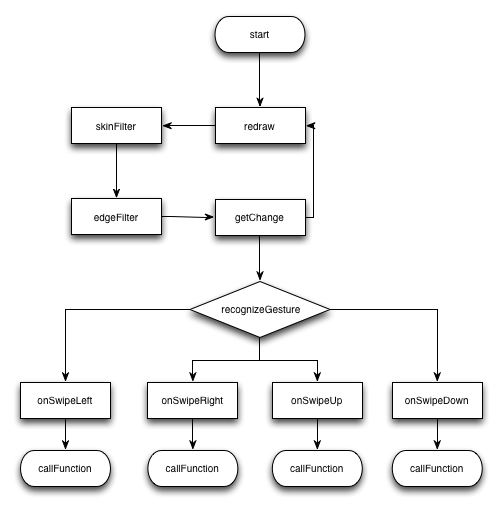
\includegraphics[width=0.8\textwidth]{diagram/motion.png}
  \caption[Algoritmus ovládania aplikácie pomocou pohybu]{
    Algoritmus ovládania aplikácie pomocou pohybu}
  \label{fig: diamotion}
\end{figure}

\paragraph{Vizualizácia} % (fold)
\label{par:zobrazenie_n_h_adu}

V aplikácii je možné pridať aj zobrazenie aktuálneho náhľadu z webovej kamery a to použitím vytvorenej direktívy pridaním atribútu ,,adaptive-motion'' ku canvas elementu. Atribút môže nadobúdať nasledujúce hodnoty:

\begin{itemize}
  \item video - zobrazí aktuálny náhľad z web kamery zariadenia, ktorého detail je zobrazený na obrázku \ref{fig: motion-video}
  \item skin - zobrazí video stream po aplikovaní filtra rozpoznania kože, ktorého detail je zobrazený na obrázku \ref{fig: motion-skin}
  \item edge - zobrazí video stream po aplikovaní filtra rozpoznania hrán, ktorého detail je zobrazený na obrázku \ref{fig: motion-edges}
\end{itemize}


% paragraph zobrazenie_n_h_adu (end)

% subsubsection pohyb (end)

\subsubsection{Gyroskop} % (fold)
\label{ssub:gyroskop}

Jednou z možností ovládania webovej aplikácie je použitie gyroskopu. Na tento prípad som vytvoril modul pomocou ktorého je možné vo webovej aplikácií skrolovať len pomocou natáčania zariadenia do strán bez ďalšej potrebnej interakcie používateľa. Cieľom je zároveň umožniť ovplyvniť samotnú rýchlosť skrolovania na základe veľkosti natočenia oproti počiatočnej pozícii zariadenia.

Modul sa inacializuje pridaním atribútu ,,adaptivescroll'' k elementu, v ktorom má prebiehať skrolovanie. Tým môže byť napríklad element ,,body'', ktorý zohľadňuje skrolovanie celej webovej stránky, alebo aj nejaký iný vnorený element. V takom prípade však skrolovanie prebieha len v rámci daného elementu.

\begin{lstlisting}
<body adaptivescroll> </body>
\end{lstlisting}

Následne stačí zavalať metódu so začatím sledovania polohy zariadenia, v ktorej sa môže upraviť ignorovaná hranica natočenia v uhloch a skrolovanie prebieha automaticky. V prípade potreby je toto sledovanie možné aj ukončiť.

Po začatí sledovania aktuálneho natočenia zariadenia sa uloží jeho počiatočná hodnota, ktorá sa používa ako relatívna hranica medzi stranami na ktoré prebieha skrolovanie. Postupným natáčaním zariadenia v smere hodinových ručičiek okolo osi beta od počiatočnej hodnoty k používateľovi sa vykonáva skrolovanie elementu smerom dolu, natáčaním na opačnú stranu od počiatočnej hodnoty prebieha skrolovanie hore.

Do úvahy pri zohľadňovaní rýchlosti skrolovania sa berie aj absolútna hodnota natočenia zariadenia od počiatočnej hodnoty zariadenia. Čím je táto hodnota väčšia, tým rýchlejšie prebieha skrolovanie. Výpočet rozdielu natočenie zohľadňuje smer rotácie a je určený na základe počiatočnej rotácie, aktuálneho natočenia a celkovej veľkosti rotácie pre danú os:

\begin{lstlisting}
var getDiff = function(startOrientation, actualOrientation, interval){
  var d1 = startOrientation - actualOrientation;
  var d2 = startOrientation - actualOrientation - interval;
  return (Math.abs(d1) < Math.abs(d2)) ? d1 : d2;
};
\end{lstlisting}

Samotný proces skrolovania prebieha vďaka číselnej zmene offsetu elementu. Plynulosť skrolovania je zaručená použitím animácii pomocou requestAnimationFrame. Tá prebieha s frekvenciou 60 fps a je časovaná priamo prehliadačom. Tej však chýba podpora v straších verziách, v takom prípade musí byť použítý manuálny časovač aplikácie.

Okrem skrolovania modul obsahuje aj ďalšie metódy onalpha, onbeta a ongamma, ktorých návratová funkcia sa zavolá vždy po zmene rotácie zariadenia a je ich možné použiť na iné potreby v aplikácii. Funkcia obsahuje parameter absolútnu zmenu pozície v uhloch od počiatočnej k aktuálnej, ktorá sa používa aj pri skrolovaní v aplikácii. Diagram navrhnutého algoritmu ovládania webovej aplikácie pomoc gyroskopu sa nachádza na nasledujúcom obrázku:

\begin{figure}[H]
  \centering
  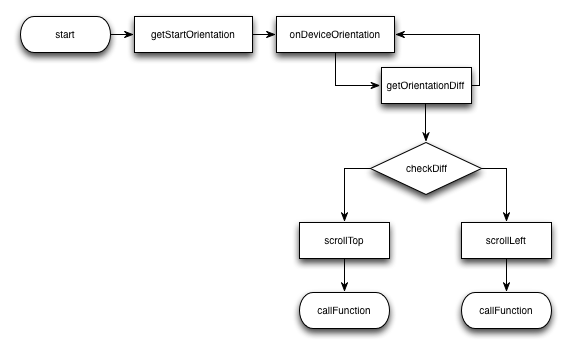
\includegraphics[width=1.0\textwidth]{diagram/scroll.png}
  \caption[Algoritmus ovládania aplikácie pomocou gyroskopu]{
    Algoritmus ovládania aplikácie pomocou gyroskopu}
  \label{fig: diascroll}
\end{figure}

% subsubsection gyroskop (end)

% subsection alternat_vne_sp_soby_ovl_dania (end)

% \newpage
\subsection{Komponenty} % (fold)
\label{sub:komponenty}

Jednou z najväčších kritík voči technike ,,responsive Web design'' je, že webové stránky sú príliš veľké a teda sa predlžuje čas ich načítania. Ale my vieme spraviť webové stránky s dobrým výkonom, len musíme vykonať prácu navyše \cite{20mb}.

Všetci by sme sa mali zaujímať o rýchlosť načítavania a mobilný výkon stránok, pretože ľudia potrebujú zážitok z rýchlosti stránok. Existuje mnoho štúdií ktoré zdôrazňujú dôležitosť rýchlosti. Viac ako polovica ľudí so zlou skúsenosťou s načítavania stránky na mobile sa nevráti späť \cite{OptimizingtheCriticalRenderingPath}. 73\% ľudí s mobilnym pripojením zažilo stránky, ktoré sú príliš pomalé, 1 sekundové spomalenie načítania vedie k poklesu o 7\% pri konverziach \cite{pagespeed}. Rýchlosť je základnou časťou našej stratégie a všetci by sa mali o ňu starať. Môžme merať jej dopad na metriky a sledovať ju.

Zároveň existuje aj mnoho druhov internetových pripojení. Rýchlosti mobilných sietí sa síce zvýšili, ale stále nám to moc nepomôže pretože časové oneskorenia sú stále príliš dlhé. Latencia je jednou z najvýznamnejších častí pri sťahovaní stránky. LTE štandart redukuje latenciu k BTS staniciam o niekoľko milisekúnd ale my stále potrebujeme vykonať viacero požiadaviek na stiahnutie dát do zariadení \cite{OptimizingtheCriticalRenderingPath}.

Čo by sme teda mali urobiť? Môžme vytvoriť znovupoužiteľné webové komponenty a podmienene načítať ich zdroje. Webové komponenty nám umožnia vytvoriť vlastné HTML elementy v prehliadači. Pomocou nich môžme rozšíriť jednoduchý element alebo za nich schovať celú aplikačnú logiku \cite{webcomponents}. Môžme vytvoriť webovú aplikáciu znovupoužiteľným a zapúzdreným spôsobom.

Dôležité sú však webové komponenty s ktorými používateľ webovej aplikácie priamo interaguje. Tieto boli skúmané najmä z hľadiska optimalizácie na rôzne zariadenia a rýchlosti pripojenia.

\subsubsection{Video} % (fold)
\label{subsub:video}

Populárnym doplnkom súčasných webový stránok je priložené video, ktoré sa často nachádza na serveroch YouTube alebo Vimeo.

Problémom je, že pri vložení videa pomocou iframe alebo embed api sa uskotočňuje množstvo dopytov na servery a prenášajú sa zbytočné dáta aj keď používateľa video nezaujíma a vôbec si ho neprehrá. Okrem zbytočne prenášaných dát sa aj znižuje výkon, nakoľko určitý čas trvá spracovanie požiadaviek.

Nasledujúce dáta sa prenesú pri zobrazení stránky, na ktorú bolo vložené video zo servera YouTube pomocou dostupného iframe API:

\begin{figure}[H]
	\centering
	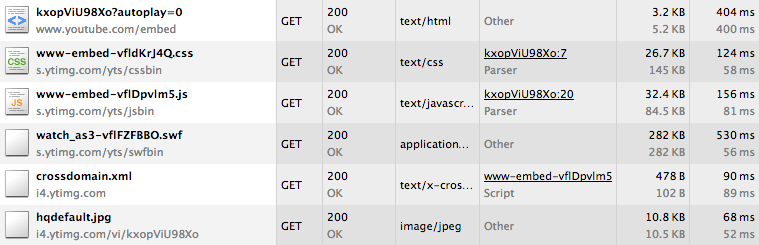
\includegraphics[width=0.8\textwidth]{img/youtube.png}
	\caption[Prenášané dáta pri požiadavke na video zo servera YouTube]{
		Prenášané dáta pri požiadavke na video zo servera YouTube}
	\label{fig: youtube}
\end{figure}

Celkovo sa vykoná 6 požiadaviek a prenesie sa 350 kB dát bez toho, aby používateľ spustil video. Podobná situácia sa opakuje aj pri požiadavke na video zo servera Vimeo pomocou iframe API.

\begin{figure}[H]
	\centering
	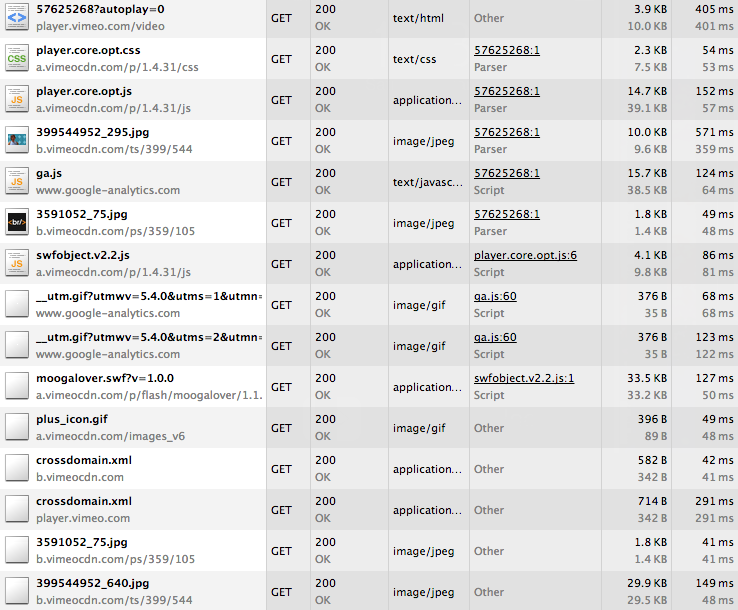
\includegraphics[width=0.8\textwidth]{img/vimeo.png}
	\caption[Prenášané dáta pri požiadavke na video zo servera Vimeo]{
		Prenášané dáta pri požiadavke na video zo servera Vimeo}
	\label{fig: vimeo}
\end{figure}

V tomto prípade sa dokonca vykoná 15 požiadaviek a prenesie sa 120 kB dát. V prípade použitia javascriptového API s HTML 5 prehrávačom videa sa síce nestiahnú flashové komponenty, ale nahradia ich rovnakoveľké javascriptové súbory.

Lepšie riešenie je použiť podmienené načítavanie. Najskôr sa načíta len obrázok videa a pridajú sa jednoduché štylistické prvky aby vytvorený element pripomínal video súbor a až po kliknutí sa urobia dopyty na vzdialený server s automatickým prehratím videa. Výhodou takéhoto riešenia je zmenšenie veľkosti dopytov a s tým spojené šetrenie dát používateľov. 

Čo sa týka získania obrázkového náhľadu videa, tak YouTube túto možnosť priamo poskytuje a záleží len od identifikátora videa. K obrázku je tak možné pristúpiť priamo. Navyše po vykonaní požiadaviek na server po kliknutí na obrázok a následnom spustení videa pomocou api sa už daný onrázok nachádza v pamäti, tak sa nemusia robiť ďalšie požiadavky. 

Samotný proces automatického spustenia YouTube videa nie je úplne jednoduchý, nakoľko nastavenie hodnoty ,,autoplay'' pri vložení elementu iframe s videom na stránku nefunguje na mobilnom prehliadači Safari, kde je táto možnosť zakázaná. V takomto prípade by sa po kliknutí na obrázok videa načítal len element s videom a aby sa samotné video začalo prehrávať očakáva sa ďalšie kliknutie. Takéto správanie je neželené a je proti používateľskému zážitku. 

Preto bolo potrebné vymyslieť lepšie riešenie. To spočíva v načítaní scriptu s javascriptovým youtube API a následným vytvorením iframe elementu s videom až pomocou neho. Takto máme prístup k programátorskému ovládaniu prehravača videa a môžme ho spustiť keď potrebujeme, teda po kliknutí na obrázok s náhľadom videa. Takéto riešenie už fungujé aj na iOS s mobilným prehliadačom Safari.

Stále však máme problém pri staršej verzii iOS 5 a menej, tam nefunguje ani programátorske spustenie videa. V tejto verzii iOS sa však ešte distribuovala predinštalovaná aplikácia na prehrávanie Youtube videí, ktorá bola v neskorších verziách odstránená a je ju možné stiahnúť z iTunes. Výhodou je, že video môžme otvoriť priamo v nej pomocou youtube url schémy. Musíme však používaný prehliadač správne detekovať a následne sa rozhodnúť, aké prehrávanie zvolíme.

Na detekovanie funkcionality otvorenia youtube videa v aplikácii pomocou systému iOS a jej zisťovaním len z pola ,,user agent'' nie je správne, nakoľko by bolo potrebné získať úplne všetky verzie systému, ktorých je mnoho, a následne porovnať s verziou zariadenia.

Lepším riešením je vytvorenie testu funkčnosti prehrávania videa, ktoré je riešené pomocou nástroja Modernizr\footnote{Modernizr \url{http://modernizr.com/} je JavaScriptová knižnica, ktorá detekuje dostupnosť natívnej imlementácie nových technológií v prehliadači.} umožňujúcim detekciu základných HTML5 a CSS3 vlastností prehliadača a vytváranie vlastných testov. Následne sa na základe výsledku testu rozhodnemu akú akciu vykonať. Problémom je, že testy sa vykonávajú po načítaní stránky a nechceme používateľovi automaticky otvoriť natívnu aplikáciu alebo ho presmerovať na stránky youtube. Preto je zvolená iná varianta a detekuje sa podbora vlastnosti, ktorá bola pridaná až v novšej verzii iOS 6. Konkrétne sa jedná o podboru jednotiek ,,vh a vw'' (viewport height a viewport width) slúžiacich na nastavenie veľkosti DOM elementu. Detekcia či je zariadenie iOS vychádza z pola user agent, ale už sa nezisťuje jej verzia.

Výsledok je taký, že po kliknutí na obrázok s náhľadom videa a vyhodnotení testu prehrávania sa začne prehrávať v prehliadači alebo v natívnej aplikácii.

V prípade Vimea je situácia trochu komplikovanejšia pretože k náhľadovému obrázku sa priamo nevieme dostať a je potrebné urobiť jednu požiadavku na API, ktorá vráti informácie o videu. Vykonanie požiadavky síca nejaký čas trvá, ale aj tak je výsledok z pohľadu prenášaný údajov lepší ako robiť požiadavku priamo na samotné video.

S prehrávaním videa zo služby vimeo je situácia podobná, neexistuje však natívna aplikácia a po klinutí na náhľad videa je používateľ v starších verziách iOS presmerovaný na stránky vimea, v novších verziách iOS a v Androide sa mu automaticky prehrá.

% subsubsection video (end)


\subsubsection{Mapy} % (fold)
\label{subsub:mapy}

Mapy podobne ako videá vytvárajú nechcené dátové prenosy, dokonca ich ešte aj prevyšujú pretože sa neprenášajú len údaje o aktuálne zobrazenej časti mapy ale aj jej okolie. Okrem nich navyše na webe neposkytujú taký plnohodnotný zážitok z prezerania ako v natívnej aplikácii. Nevýhodou je aj nemožnosť posúvania webovej stránky pokiaľ je element s mapou väčší ako je rozlíšenie displeja mobilného zariadenia, lebo eventy sú zachytávané mapou a posúva sa tá.

Používateľ nemusí chcieť okamžite interagovať s mapou a v takomto prípade ho zbytočne zaťažuje. Výhodnejšie je tak zobraziť len náhľad mapy, ktorý sa načíta rýchlejšie pretože šetrí prenášané dáta, a pokiaľ sa používateľ chce dozvedieť viac, tak len jednoducho na mapu klikne. V takomto prípade sa mu automaticky načíta plne interaktívna mapa. Na zobrazenie náhľadu mapy existuje API v službe google maps\footnote{\url{https://developers.google.com/maps/documentation/staticmaps/}}, takže je možné využiť priamo to. Nevýhodou je, že počet požiadaviek za deň, ktoré sú zadarmo, je obmedzený, po získaní API kľúča je možné ich spraviť 25000, ďalšie sú spoplatňované.

Rozšírením na mobilných zariadeniach iOS je možnosť otvorenia mapy priamo v natívnej aplikácii, ktorá prináša ešte väčší používateľský zážitok ako zobrazenie na webe. To je uskutočňované pomocou url schémy. V starších verziách iOS sa nachádzala natívna aplikácia na Google API a bola vyvolaná otvorením odkazu \url{http://maps.google.com/}, kde bolo možné zadávať parametre zobrazenia.


\begin{figure}[H]
  \centering
  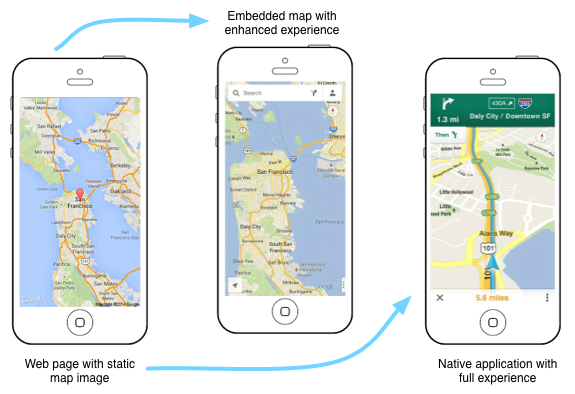
\includegraphics[width=0.8\textwidth]{img/maps.png}
  \caption[Podmienené otváranie máp]{
    Podmienené otváranie máp}
\end{figure}

S príchodom iOS 6 bola aplikácia nahradená vlastnom Apple aplikáciou, na ktorej spustenie sa zmenila aj url schéma a pôvodná otvorí mapu len v prehliadači. Výhodou je, že na starších, respektíve nepodporovaných zariadeniach nastáva presmerovanie na stránky Google a tak na rovnakom odkaze funguje spúšťanie aj pôvodnej aplikácie. Nová url schéma má tvar \url{http://maps.apple.com/}.

% subsubsection mapy (end)


\subsubsection{Lightboxy} % (fold)
\label{subsub:lightboxy}

Lightbox je technika umožňujúca zobrazovať webový obsah v modálnych oknách nachádzajúcich sa nad úrovňou pôvodnej stránky.

Hlavným problémom použitia ,,lightboxov'' na mobilných zariadeniach je nesprávne zobrazovanie stránok pokiaľ nové okno je väčšie ako displej. V takomto prípade by bolo vhodnejšie používateľa presmerovať priamo na novú stránku.

% subsubsection lightboxy (end)

\subsubsection{Otvorenie v aplikácii / Stiahnutie aplikácie} % (fold)
\label{ssub:otvorenie_v_aplik_cii}

V súčasnosti sme opklopovaný množstvom informačných zdrojov, ktoré sa zväčša nachádzajú na internete dostupné na konkrétnej webovej adrese. Na tieto zdroje existuje množstvo odkazov z rôznych webových stránok, sociálnych sietí či mobilných aplikácii, ktoré zobrazia ich obsah v prehliadači.

\begin{fancybox}
\textit{,,Links don’t open apps.'' Jason Grigsby} \cite{links}
\end{fancybox}

Webové odkazy neotvárajú natívne aplikácie, čo je technicky pravda, no realita je trochu odlišná. Prepojenie webovej časti aplikácie s natívnou umožňuje otvárať komplexnejšie úlohy, na ktoré je vo webe nedostatočny výkon, priamo v natívnom kóde. To umožní plynulejší chod aplikácie a lepší používateľský zážitok.

Prepájanie aplikácii sa uskutočňuje pomocou ,,custom url schémy'' \cite{urlscheme}, ktorá je špecifická pre jednotlivé operačné systémy zariadení. Nevýhodou vlastných odkazov je, že pokiaľ používateľ nemá nainštalovanú aplikáciu, tak po kliknutí sa objaví celkom nepekná chybová hláška.

\begin{figure}[H]
	\centering
	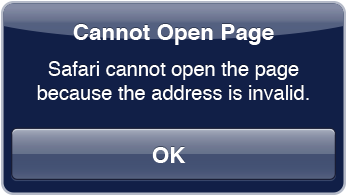
\includegraphics[width=0.35\textwidth]{img/customerror.png}
	\caption[Chybová hláška po otvorení custom URL schémy, pokiaľ aplikácia neexistuje]{
		Chybová hláška po otvorení custom URL schémy, pokiaľ aplikácia neexistuje \cite{customscheme}.\\
		Prevzaté z http://www.lukew.com/ff/entry.asp?1654}
	\label{fig: customerror}
\end{figure}

Lepším riešením je detekovanie, či si používateľ stiahol natívnu aplikáciu a odkaz na otvorenie v nej vytvoriť až potom, čo je overenie úspešné. Pokiaľ by nebolo, tak by sa mohlo zobraziť tlačítko na stiahnutie natívnej aplikácie, ktoré opäť musí byť prispôsobené platforme na ktorej na stránku prispôsobujeme, pokiaľ nechceme používateľa zahltitť všetkými platformami ktoré podporujeme.

Samotný proces detekcie či má používateľ nainštalovanú našu aplikáciu vôbec nie je triviálny, pretože na webe neexistuje žiadne dostupné API, ktoré by zahrňovalo všetky platformy. Apple síce vydal možnosť otvorenia aplikácie pomocou ,,Smart Banners'', ale až v iOS 6 a tak táto možnosť nie je úplne použiteľná.

\begin{figure}[H]
	\centering
	
\includegraphics[width=0.5\textwidth]{img/smartappbanner.png}
	\caption[Otvorenie natívnej aplikácie v iOS 6]{
		Otvorenie natívnej aplikácie v iOS 6 \cite{smartappbanner}.\\
		Prevzaté z http://developer.apple.com/}
	\label{fig: smartappbanner}
\end{figure}

Navyše ,,smart banner'' je priamo definovaný v html meta tagu aplikácie. Na stránke existuje len jeden ktorý volá url schému aplikácie a aj ten má prednastevený vzhľad v podobne okna v hornej časti obrazovky. Keby chceme vlastnú natívnu aplikáciu zavolať z viacerých častí webovej, prípadné volať viacero natívnych aplikácií, tak toto riešenie je nepostačujúce. Nemôže byť upravané vlastným potrebám.

Jediné možné riešenie je len v spolupráci s natívnou aplikáciou, aj tak sa však musí vyvolať otvorenie stránky v prehliadači, kde sa dá už do cookies alebo lokálneho úložiska programátorksy zapísať existencia aplikácie. Vytvorenie samotného ,,webView'' komponentu s webovou stránkou vrámci aplikácie a následné zatvorenie nestačí. Prehliadač má oddelené úložiská stránok pre rôzne typy prístupov ako sú s internetový prehliadač, aplikácia a v iOS aj pre otvorenie internetovaj stránky z plochy. Možnosť ako tento proces zamaskovať je skrytá v procese registrácie, keď po otvorení aplikácie a zaregistrovaní pošleme používateľovi e-mail s potvrdzujúcim odkazom, ktorý otvorí webovú stránku v prehliadači.


% subsubsection otvorenie_v_aplik_cii (end)

% subsection komponenty (end)

\newpage
\subsection{Nástroje} % (fold)
\label{sub:n_stroje}

\subsubsection{Detekcia} % (fold)
\label{ssub:detekcia}

Pre potreby rozpoznávania platformy v aplikácii bol vytvorený modul detekcie podľa jedinečného ,,user agent'' textu. Modul umožňuje detekovať iOS a Android zariadenia. Rozpoznávanie prebieha na základe regulárneho výrazu, kde pri metóde detekcie iOS zariadenia sa kontroluje výsky slov ,,iPhone'', ,,iPad'' alebo ,,iPod'', ktoré jedinečne definujú platformu. Pri Android zariadeniach je detekcia jednoduchšia, pretože stačí ak sa v identifakačnom texte nachádza slovo ,,Android''. Príklad metódy detekcie má nasledujúci tvar:

\begin{lstlisting}
var isAndroid = function(userAgent){
  return (/(Android)/gi).test(userAgent);
}
\end{lstlisting}

Pri konfigurácii webovej aplikácie je možné aj aktálny ,,user agent'' text nahradiť vlasnou hodnotou, takže prehliadač sa vždy môže správať ako požadované zariadenie. Problém pri detekcii môže nastať, pokiaľ by user agent už bol raz nahradený používateľom, respektíve by sa prestali používať súčasné identifikátory. Potom by sa detekovala nesprávna platforma.

% subsubsection detekcia (end)

% subsection n_stroje (end)

% section n_stroj_na_overenie (end)
\newpage
\section{Overenie} % (fold)
\label{sec:overenie}

Detekovali sme niekoľko vstupných metód, webových komponentov a overovali ktoré z nich poskytujú lepší používateľský zážitok pre návštevníkov webových stránok ako aj pre samotných webových vývojárov. Na obe adaptívne vstupnú metódy aj webové komponenty boli vytvorené série experimentov. Na preukázanie užitočnosti navrhnutého konceptu sme navrhli a implementovali niekoľko opakovane použiteľných modulov a komponentov. Overenie jednotlivých častí projektu je riešené vytvorením prototypových aplikácií ku každému vytvorenému modulu a pomocou získanej spätnej väzby z komunity. Všetky súčasti boli vytvorené pod open source licenciou a sú dostupné na GitHube. Implementované sú nasledujúce súčasti systému:

\begin{itemize}
  \item \textbf{angular-adaptive/adaptive-speech}\\
    modul na ovládanie aplikácie pomocou reči
  \item \textbf{angular-adaptive/adaptive-scroll}\\
    modul na ovládanie aplikácie pomocou gyroscopu
  \item \textbf{angular-adaptive/adaptive-motion}\\
    modul na ovládanie aplikácie pomocou pohybu
  \item \textbf{angular-adaptive/adaptive-detection}\\
    modul na detekovanie zariadenia
  \item \textbf{angular-adaptive/adaptive-googlemaps}\\
    webový komponent google máp
  \item \textbf{angular-adaptive/adaptive-youtube}\\
    webový komponent youtube videí

  \item \textbf{Gyrocopter}\\
    rozšírenie do Chrome Developer Tools na emulovanie gyroskopu
  \item \textbf{speech-synthesis}\\
    polyfill rečovej syntézy
\end{itemize}

Pre vytvorené webové komponenty sme sledovali množstvo ušetrených dát, merali zrýchlenia načítavania webových stránok či počty vykonaných dopytov na server pre rôzne druhy internetových pripojení. Pre adaptívne vstupné metódy sme zisťovali najmä záujem o jednotlivé druhy alternatívnych ovládaní webových stránok. Z komunity sme získali množstvo spätnej väzby, ktorá nám taktiež pomohla overiť navrhnutý koncept a ďalej prispôsobiť riešenia. Podľa analytických nástrojov sa experimentov zúčastnili desaťtisíce používateľov a vývojárov.

\newpage
\subsection{Adaptívne vstupné metódy} % (fold)
\label{sub:adapt_vne_ovl_dacie_met_dy}

Adaptívne vstupné metódy poskytujú alternatívne spôsoby ovládania webových aplikácií. Experimentovali sme ovládaním webových aplikácií pomocou rečových povelov, pohybu detekovaného pomocou gyroskopu a video kamery.

\subsubsection{Modul adaptive-speech} % (fold)
\label{sub:adaptive_speech}

Ovládanie pomocou reči bolo demonštrované vytvorením modulu adaptive-speech \footnote{\url{https://github.com/angular-adaptive/adaptive-speech}} a prototypovej aplikácie nad existujúcim systémom TodoMVC \footnote{\url{http://todomvc.com/}}, ktorý demonštruje vytvorenie todo aplikácie v rôznych javascriptových frameworkoch. 

Vytvorený experiment založený na našom module poskytoval ovládanie aplikácie todo listu. Po spustení aplikácie a potvrdení prístupových povolení od používateľa k používaniu mikrofónu nie je potrebné ďalšia interakcia okrem zadávania rečových príkazov, nakoľko prebieha kontinuálne rozpoznávanie reči. Celkovo sa v ňom rozpoznávalo 7 presných rečových povelov a 9 rečových povelov založených na použití regulárnych výrazov. V aplikácii je tak umožnené pridávanie novej úlohy, jej označenie za splnenú alebo úplne odstránenie zo zoznamu. Taktiež je umožnené prechádzanie medzi jej jednotlivými časťami a prepinaním zobrazenia všetkých úlohoch, aktívnych úloh a splnených úloh. Rovnako je umožnené pomocou rečového príkazu aj vymazať všetky splnené úlohy. Vytvorená demo aplikácia je znázornená na nasledujúcom obrázku:

\begin{figure}[H]
  \centering
  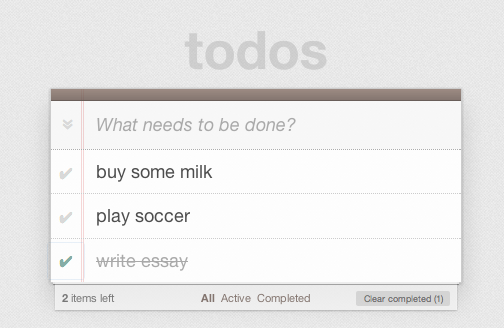
\includegraphics[width=0.75\textwidth]{img/adaptivespeech.png}
  \caption[Prototypová aplikácia vytvoreného modulu adaptive-speech]{
    Prototypová aplikácia vytvoreného modulu adaptive-speech}
  \label{fig: adaptivespeech}
\end{figure}

K samotnému modulu som získal veľké množstvo spätnej väzby a je v komunite najpopulárnejší spomedzi ostatných alternatívnych metód ovládania aplikácie. Samotného experimentu sa zúčastnili tisíce používateľov. Pomocou hlasového ovládania sa dá v aplikácii dosiahnuť množstvo vecí a pomocou neho vieme ovládať kompletnú aplikáciu bez použitia ostatných vstupných metód. Dokonca vieme aplikáciu ovládať vo viacerých jazykoch. Najväčším problémom v súčasnosti je však nie úplne správne rozpoznanie hovorených príkazov. Na jeho zmiernenie ale vieme použiť regulárne výrazy alebo nápravu výrazov v slovníku od používateľa.

Podpora ovládania pomocou reči v prehliadačoch v súčasnosti ešte nie je veľmi rozšírená a vyzerá nasledujúco:

\begin{table}[H]
  \begin{tabular}{ | l | l | l | l | l | l | l | l |}
    \hline
    IE & Firefox & Chrome & Safari & Opera & iOS Safari & Android & Chrome for Android \\ \hline
    nie & nie & 25.0 & nie & nie & nie & nie & 31.0  \\
    \hline
  \end{tabular}
  \caption[Podpora rozopoznávania reči]{Podpora rozopoznávania reči}
\end{table}

S použitím rozpoznania reči súvisí aj rečová syntáza, vďaka ktorej vieme interagovať pomocou reči a ešte viac zvýšiť používateľský zážitok. Nativná podpora však tiež nemá širokú podporu a pre tieto potreby bol vytvorený polyfill vďaka ktorému vieme rečovú syntézu nahradiť pomocou Audio elementu a prehravaním audia zo služby Google Translate. Porovnanie podpory v prehliadačoch vyzerá nasledujúco:

\begin{table}[H]
  \begin{tabular}{ | l | l | l | l | l | l | l | l |}
    \hline
    IE & Firefox & Chrome & Safari & Opera & iOS Safari & Android & Chrome for Android \\ \hline
    nie & nie & 33.0 & 7.0 & nie & 7.0 & nie & 33.0  \\
    \hline
  \end{tabular}
  \caption[Natívna podpora rečovej syntézy]{Natívna podpora rečovej syntézy}
\end{table}

\begin{table}[H]
  \begin{tabular}{ | l | l | l | l | l | l | l | l |}
    \hline
    IE & Firefox & Chrome & Safari & Opera & iOS Safari & Android & Chrome for Android \\ \hline
    9 & áno & áno & áno & áno & 4.0 & 2.3 & áno  \\
    \hline
  \end{tabular}
  \caption[Podpora polyfillu rečovej syntézy]{Podpora polyfillu rečovej syntézy}
\end{table}

% subsubsection adaptive_speech (end)

\subsubsection{Modul adaptive-scroll} % (fold)
\label{sub:adaptive_scroll}

Ovládanie pomocou gyroskopu bolo demonštrované vytvorením modulu adaptive-scroll \footnote{\url{https://github.com/angular-adaptive/adaptive-scroll}} a prototypovej aplikácie. V aplikácii je možné po spustení skrolovať pomocou natáčania zariadenia do strán. Skrolovanie prebieha na základe veľkosti uhlu natočenia zariadenia oproti počiatočnej polohe, čím je rozdiel väčší, tým sa vo webovej aplikácii skroluje rýchlejšie. Na skrolovanie v aplikácii nie je potrebná ďalšia interakcia používateľa, napríklad pomocou dotyku. 

Experimentu sa zúčasnili tisíce používateľov a je podporovaný vo veľkom počte prehliadačoch, konkrétne v nasledujúcich:

\begin{table}[H]
  \begin{tabular}{ | l | l | l | l | l | l | l | l |}
    \hline
    IE & Firefox & Chrome & Safari & Opera & iOS Safari & Android & Chrome for Android \\ \hline
    11 & áno & áno & nie & áno & 4.2 & 3.0 & áno  \\
    \hline
  \end{tabular}
  \caption[Podpora získavania orientácie v prehliadačoch]{Podpora získavania orientácie v prehliadačoch}
\end{table}

Pomocou modulu vieme zvýšiť používateľský zážitok, nevieme však ovládať kompletnú webovú aplikáciu ako v prípade rečových povelov. Po vytvorení modulu a testovaní na zariadeniach sa navyše zistili problémy v skutočnej implementácii udalostí natáčania zariadenia v rôznych prehliadačoch. W3C špecifikácia orientácie zariadenia uvádza nasledovné:

\begin{itemize}
  \item os X je rovnobežná na rovinu zeme, kladné hodnoty má v smere na východ, záporné na západ
  \item os Y je rovnobežná na rovinu zeme, kladné hodnoty má v smere na sever, záporné na juh
  \item os Z je kolmá na rovinu zeme, kladné hodnoty má v smere od zeme, záporné smerom k zemi
\end{itemize}

Rotácia by mala byť popísaná pravidlom pravej ruky, teda kladné hodnoty rotácie sú v smere hodinových ručičiek okolo osí.

Nasledujúce tabuľky ukazujú, kde sa nachádzajú nulové body pre jednotlivé osi, aké hodnoty nadobúda rozsah rotácie a či je dodržané pravidlo pravej ruky.

Pravidlo pravej ruky (PPR) hovorí: 

\begin{fancybox}
\textit{,,Kladné hodnoty rotácie sa zvyšujú pri rotovaní okolo osi v smere hodinových ručičiek pri ukazovaní smerom na narastajúcu kladnú hodnotu smerovej osi.'' W3C \cite{deviceorientation}}
\end{fancybox}


Táto definícia je však protichodná s hodnotami kompasu. Pri rotácii okolo osi Z v smere rotácie kompasu sa hodnoty rotácie znižujú a nie narastajú. To je však spôsobené pohľadom do záporných hodnôt osi Z.


\paragraph{Alpha} % (fold)
\label{par:alpha}

Rotácia okolo osi Z nadobúda hodnoty rotácie alpha. V špecifikácii je nejasne definové aké by mali byť východiskové hodnoty, čo vo výsledku prináša rôzne implementácie rotácie v prehliadačoch. To spôsobuje zmätok nakoľko zo špecifikácie nie je jasné, na akú stranu by mal ukazovať nulový bod. Dá sa odpozorovať podľa pravidla pravej ruky, že 0 stupňov ukazuje smerom na sever, pretože implementovaných 90 stupňov ukazuje na východ.

Rozsah hodnôt bol testovaný pri držaní zariadenia v horizontálnej polohe a vycentrovaní smerom k nulovému bodu, keď hodnota rotácie bola 360 stupňov. Pozorované boli nasledujúce hodnoty:

\begin{table}[H]
  \begin{tabular}{ | l | l | l | l |}
  \hline
              & Nulový bod  & PPR   & Rozsah \\ \hline
  Reference   & Sever (0)   & A     & [0, 360] \\  
  iOS Chome   & Východ (90)   & A     & [0, 360] \\  
  iOS Safari  & Východ (90)   & A     & [0, 360] \\  
  Android & & & \\  
  Chrome      & Sever (0)   & A     & [0, 360] \\  
  Stock       & Západ (270)  & A     & [0, 360] \\  
  Firefox     & Sever (0)   & N     & [0, 360] \\
  \hline
  \end{tabular}
  \caption[Alpha rotácia gyroskopu]{Alpha rotácia gyroskopu}
\end{table}

% paragraph alpha (end)


\paragraph{Beta} % (fold)
\label{par:beta}

Rotácia okolo osi X nadobúda hodnoty rotácie beta. Špecifikácia definuje nulový bod ako horizontálnu polohu. Všetky testované prehliadače majú implementovaný smer osi rotácie správne, problémy však nastávajú pri rozsahu rotačných hodnôt.

Rozsah bol testovaný pri držaní zariadenia v horizontálnej polohe, čo je nulový bod. Zariadenie bolo potom otáčané okolo osi X o 90 stupňov tak, že displej zariadenia smeroval k pozorovateľovi. Potom nasledovalo otáčanie o ďalších 90 stupňov tak, že displej bol smerom k zemi. Na koniec nasledovala rotácia zvyšných 180 stupňov smerom do počiatočnej polohy, čím sa rotácia dokončila.


\begin{table}[H]
  \begin{tabular}{ | l | l | l | l | l |}
  \hline
              & Nulový bod    & PPR   & Rozsah         & Poznámky\\ \hline
  Reference   & Horizontálne   & A     & [0, -180|180] & \\  
  iOS Chome   & Horizontálne   & A     & [-90, 90]     & Plný rozsah rotácie nie je podporovaný. \\  
  iOS Safari  & Horizontálne   & A     & [-90, 90]     & Plný rozsah rotácie nie je podporovaný. \\  
  Android & & & & \\  
  Chrome      & Horizontálne   & A     & [-90, 90]     & Plný rozsah rotácie nie je podporovaný. \\  
  Stock       & Horizontálne   & A     & [-90, 90]     & Plný rozsah rotácie nie je podporovaný. \\  
  Firefox     & Horizontálne   & N     & [0, 180|-180] & Rotácie pokračuje naspäť na začiatok \\
  \hline
  \end{tabular}
  \caption[Beta rotácia gyroskopu]{Beta rotácia gyroskopu}
\end{table}

V iOS zariadeniach rovako ako v Android prehliadači a Chrome pre Android hodnoty rotácie od počiatku stúpajú správne. Ale keď rotácia nadobudne svoje maximum, čo je 90 a -90 stupňov, tak jej hodnoty začnú postupne klesať. Nie je tak podporovaný celý rozsah rotácie.

Vo Firefoxe pre Android je rotácia implementovaná opačným smerom a nie je dodržané špecifikované pravidlo pravej ruky. Je však podporovaný celý rozsah rotácie. Najskôr klesne k hodnote -180 stupňov, čo sa pri pokračujúcej rotácii zmení na kladnú hodnotu a potom klesá k nule.


% paragraph beta (end)

\paragraph{Gamma} % (fold)
\label{par:gamma}

Rotácia okolo osi Y nadobúda hodnoty rotácie gamma. Špecifikácia definuje nulový bod v horizontálnej polohe. Ale aj v tomto smere rotácie sú problémy s rozsahom rotácie, ale to je spôsobené najmä samotnou špecifikáciou zo strany W3C, nakoľko v nej sa nachádza rozsah len od -90 po 90 stupňov, čo je celkovo 180 a nie je tak pokryté celé otočenie.

Rozsah hodnôt bol testovaný pri držaní zariadenia v horizontálnej polohe a natočením na nulový bod. Zariadenie bolo potom otáčané okolo osi Y o 90 stupňov v smere hodinových ručičiek tak, že jeho displej smeroval vpravo. Potom nasledovalo otočenie o ďalších 90 stupňov tak, že zariadenie smerovalo dolu. Na koniec sa dokočilo zostávajúcich 180 stupňov rotácie do pôvodného stavu.

\begin{table}[H]
  \begin{tabular}{ | l | l | l | l | l |}
  \hline
              & Nulový bod    & PPR   & Rozsah         & Poznámky\\ \hline
  Reference   & Horizontálne   & A     & [0, 90|-90]   & Zlá definícia od W3C \\  
  iOS Chome   & Horizontálne   & A     & [0, 180|-180] & Plný rozsah rotácie nie je podporovaný \\  
  iOS Safari  & Horizontálne   & A     & [0, 180|-180] & Plný rozsah rotácie nie je podporovaný. \\  
  Android & & & & \\  
  Chrome      & Horizontálne   & A     & [0, 270|-90]  & Upravený rozsah rotácie definuje natočenie \\  
  Stock       & Horizontálne   & A     & [0, 270|-90]  & Upravený rozsah rotácie definuje natočenie \\  
  Firefox     & Horizontálne   & N     & [0, -90|90]   & Rozsah rotácie pokračuje naspäť na začiatok \\
  \hline
  \end{tabular}
  \caption[Gamma rotácia gyroskopu]{Gamma rotácia gyroskopu}
\end{table}

Zlá definícia rotácie od W3C špecifikuje rotáciu len po hodnotu 90 stupňov z horizontálnej polohy, čo spôsobuje problémy pri väčšom natočení zariadenia.

V iOS rotácia nadobúda nulový bod v horizontálnej polohe s displejom smerujúcim hore. Otočením zariadenia okolo osi Y tak, že obrazovka bude smerovať smerom dole bude aktuálne gamma natočenie nadobúdať hodnotu 180, respektíve -180 stupňov. Ak sa rotácia uskutočňuje v smere hodinových ručičiek, tak hodnoty rotácie sa postupne zvyšujú v kladných číslach. Ak rotácia ide opačným smerom proti smeru hodinových ručičiek, tak hodnoty rotácie sa zmenšujú. Pri natočení zariadenia smerom na bok lavou stranou hore je hodnota rotácia 90 stupňov, na opačnej strane pri smerovaní pravej hrany smerom hore je to -90 stupňov.

Chrome pre Android a vstavaný Android prehliadač majú spravné hodnoty rotácie od -90 po +90 stupňov. Ale po natočení zariadenia o viac ako 90 stupňov v smere hodinových ručičiek hodnota rotácie naďalej stúpa až po hodnotu 270 stupňov, čo je zároveň aj hodnota -90. Toto poskytuje možnosť presne vedieť veľkosť natočenia zariadenia.

Firefox má aj pri rotácii okolo osi Y podobný problém, a to je že hodnoty sú opačné a nedodržiava špecifikované pravidlo pravej ruky. Rozsah je správny, ale rotácie v smere hodinových ručičiek nadobúdajú záporné hodnoty a naopak.

% paragraph gamma (end)


\paragraph{Gyrocopter} % (fold)
\label{par:gyrocopter}

Na vyriešenie problémov pri vývoji webových aplikácii spôsobených rôznymi implementáciami rotácii v prehliadačoch som vytvoril rozšírenie Gyrocopter pre prehliadač Chrome \footnote{Dostupné na stiahnutie z Chrome Web Store \url{https://chrome.google.com/webstore/detail/gyrocopter/oooalfgemajfclliinfcdkifafmcfjop}}. Hlavným cieľom rozšírenia je umožniť zvoliť si simuláciu konkrétneho prehliadača a dynamicky meniť rotáciu zariadenia bez potreby testovania funkcionality na reálnom zariadení. Podobná funkcionalita sa už nachádza v developerských nástrojoch prehliadača Chrome, ale tam je možné len manuálne zadať hodnoty rotácie bez znalosti skutočných rozsahov a náhľadu natočenia zariadenia.

Toto rozšírenie umožňuje simulovať udalosti ktoré nastanú pri rotácii zariadenia, pričom používateľ môže natáčať zariadenie vo všetkých troch osiach. Rozšírenie je implementované pre vývojárov priamo do prostredia ,,Chrome Developer Tools''.

Nakoľko hodnoty rotácii sú implementované v prehliadačoch rôzne, tak používateľ má na výber zvoliť si podľa akej implementácie chce vyvolávať udalosti rotácie. Simulovanými prehliadačmi na výber sú:

\begin{itemize}
  \item W3C špecifikácia
  \item iOS Safari (Chrome používa web view)
  \item Android Chrome
  \item Android prehliadač
  \item Firefox pre Android
\end{itemize}

Samotné používateľské rozhranie rozšírenia obsahuje náhľad aktuálnej rotácie zariadenia na ktorom je možné zmeniť aktuálne simulovaný prehliadač. Pod ním sa nachádzajú uhly natočenia alpha, beta a gamma, ktoré je možné meniť. Tieto obsahujú pre jednotlivé prehliadače rozsahy a smer natočenia. Pri zmene rotácie na jednotlivých osiach sa zmena automaticky prejaví aj na náhľade zariadenia. 

\newpage
Vytvorená prototypová aplikácia na skrolovanie spolu s rozšírením Gyrocopter sú znázornené na nasledujúcom obrázku:

\begin{figure}[H]
  \centering
  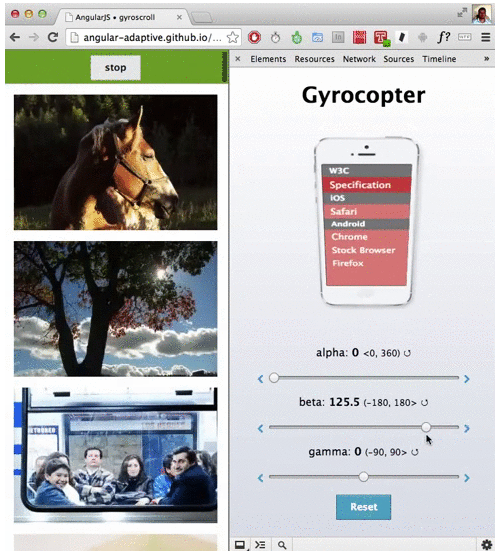
\includegraphics[width=0.6\textwidth]{img/adaptivescroll.png}
  \caption[Prototypová aplikácia vytvoreného modulu adaptive-scroll a rozšírenie Gyrocopter]{
    Prototypová aplikácia vytvoreného modulu adaptive-scroll a rozšírenie Gyrocopter}
  \label{fig: adaptivescroll}
\end{figure}

% \begin{figure}[H]
%   \centering
%   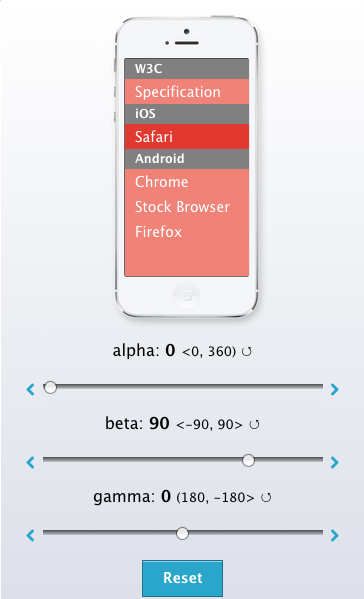
\includegraphics[width=0.35\textwidth]{img/gyrocopter.png}
%   \caption[Gyrocopter - gyroskop simulátor]{
%     Gyrocopter - gyroskop simulátor}
%   \label{fig: gyrocopter}
% \end{figure}

Po výbere, respektíve zmene prehliadača, ktorý sa má simulovať, sa automaticky prepočítajú rozsahy pre jednotlivé uhly otáčania. Zároveň sa upravia na nich aj aktuálneho hodnoty natočenia bez toho, aby sa musela znázornená rotácia zariadenia meniť.


% paragraph gyrocopter (end)

% subsubsection adaptive_scroll (end)

\subsubsection{Modul adaptive-motion} % (fold)
\label{sub:adaptive_motion}

Ovládanie pomocou pohybu bolo demonštrované vytvorením modulu adaptive-motion \footnote{\url{https://github.com/angular-adaptive/adaptive-motion}} a prototypovej aplikácie. V nej je umožnené sledovanie používateľa a možnosť výberu jeho vizualizácie, či už klasický obraz alebo upravený zobrazením len detekovaním jeho kože alebo detekciou hrán. V aplikácii prebieha kontinuálne rozpoznávanie používateľa a postupne sa vypisujú rozpoznané gestá, pričom posledné rozpoznané gesto sa zakaždým zvýrazní. Vytvorená prototypová aplikácia je znázornená na nasledujúcom obrázku:

\begin{figure}[H]
  \centering
  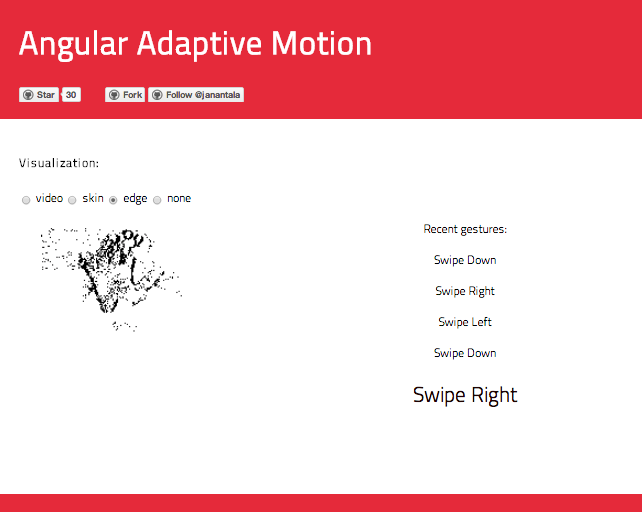
\includegraphics[width=0.6\textwidth]{img/adaptivemotion.png}
  \caption[Prototypová aplikácia vytvoreného modulu adaptive-motion]{
    Prototypová aplikácia vytvoreného modulu adaptive-motion}
  \label{fig: adaptivemotion}
\end{figure}

Experimentu sa opäť zúčasnili tisíce používateľov a vytvorený modul je podporovaný v týchto konkrétnych prehliadačoch:

\begin{table}[H]
  \begin{tabular}{ | l | l | l | l | l | l | l | l |}
    \hline
    IE & Firefox & Chrome & Safari & Opera & iOS Safari & Android & Chrome for Android \\ \hline
    nie & 17 & 21 & nie & 18 & nie & nie & 33  \\
    \hline
  \end{tabular}
  \caption[Podpora prístupu ku kamere v prehliadačoch]{Podpora prístupu ku kamere v prehliadačoch}
\end{table}

Použitím modulu vieme zvýšiť používateľský zážitok, nedokážeme však len pomocou neho ovládať celú webovú aplikáciu. Preto sa dá použiť len ako doplnková metóda interakcie čomu nasvädčuje aj získaný ohlas z komunity. Navyše vo svetlých a tmavých scénach môžu nastať problémy pri detekcii.

% subsubsection adaptive_motion (end)

% subsection adapt_vne_ovl_dacie_met_dy (end)


\newpage
\subsection{Adaptívne webové komponenty} % (fold)
\label{sub:webov_komponenty}

Pri adaptívnych webových komponentoch sme sledovali rýchlosti načítavania stránok, počty uskutočnených dopytov na server, množstvo prenášaných dát a rýchlosť zostovenia DOM stromu. Rýchlosti sme porovnávali s použitím vytvorených modulov a bez použitia pri vývoji klasickým spôsobom. Testovanie prebiehalo v rôznych podmienkach s použitím internetových pripojení s nasledujúcimi konfiguráciami:

\begin{table}[H]
  \begin{tabular}{ | l | l | l | l |}
    \hline
    Pripojenie & Dátový tok & Latencia & Stratené pakety \\ \hline
    2G & 240 kbps & 400 ms & 5 \%  \\  \hline
    3G & 780 kbps & 100 ms & 2 \%  \\ \hline
    4G & 20 Mbps & 50 ms & 1 \%  \\ \hline
    Broadband & 100 Mbps & 5 ms & 0 \%  \\
    \hline
  \end{tabular}
  \caption[Konfigurácie internetových pripojení]{Konfigurácie internetových pripojení}
\end{table}

Emulácia internetového pripojania prebiahala pomocou programu ,,Network Lint Conditioner'' a ďalej sa uvádzajú priemerné namerané hodnoty z 10 experimentov spolu so smerodajnými odchýlkami pre jednotlivé druhy internetového pripojenia.

\subsubsection{Modul adaptive-youtube} % (fold)
\label{sub:adaptive_youtube}

Webový komponent youtube videa bol demonštrovaný vytvorením modulu adaptive-youtube \footnote{\url{https://github.com/angular-adaptive/adaptive-youtube}} a demo aplikácie. V aplikácii je umožnené meniť automatické načítavanie videa. Pokiaľ sa pristupuje z mobilného zariadenia a pomalého pripojenia na internet, tak sa zobrazí len náhľad videa v podobe obrázku. Až po kliknutí na video sa dotiahne samotné video a začne sa prehrávať, respektíve video sa otvorí v natívnej mobilnej aplikácii.

Použitím vytvoreného modulu vieme ušetriť mnoho dát a zároveň aj znížiť množstvo dopytov na servery. Porovnanie priemerného množstva spotrebovaných dát a vytvorených dopytov pre jedno youtube video je zobrazené v nasledujúcej tabuľke:

\begin{table}[H]
  \begin{tabular}{ |c|c|c|c| }
    \hline
    & Embed video & Vytvorený modul \\ \hline
    Počet požiadaviek na server & 9 & 6 \\  \hline
    Množstvo prenesených dát  & 1517 KB & 389 KB  \\
    \hline
  \end{tabular}
  \caption[Množstvo požiadaviek a prenesených dát pre youtube video]{Množstvo požiadaviek a prenesených dát pre youtube video}
\end{table}

Z toho je zrejme, že použitím vytvoreneho modulu sa zrýchli aj načítavanie webovej stránky. Porovnanie načítavania stránky s použitím klasického prístupu vloženia videa a použitím nášho modulu spolu s jednotlivými uskutočnenými požiadavkami sa nachádza na nasledujúcich obrázkoch:

\begin{figure}[H]
  \centering
  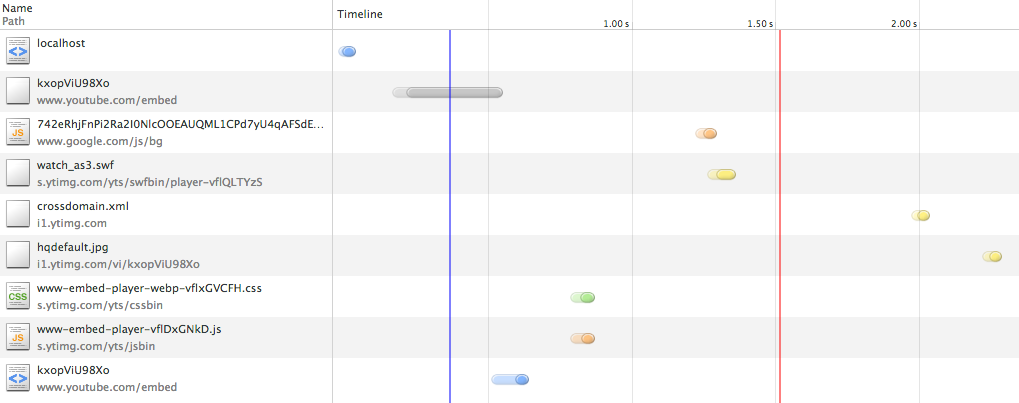
\includegraphics[width=0.9\textwidth]{img/load/timeline-y-e.png}
  \caption[Časová os načítavania stránky s použitím youtube embed videa]{
    Časová os načítavania stránky s použitím youtube embed videa}
  \label{fig: timeline-y-e}
\end{figure}

\begin{figure}[H]
  \centering
  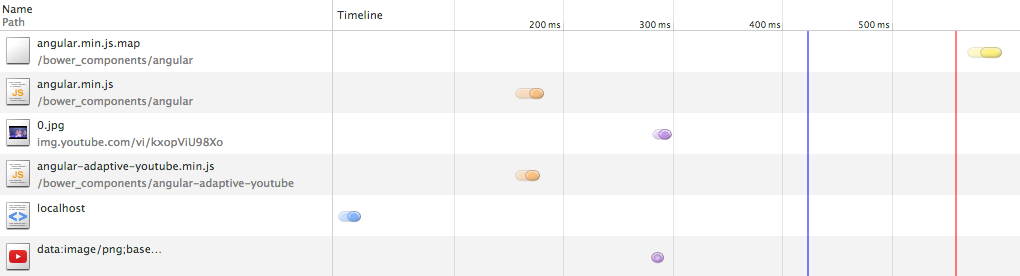
\includegraphics[width=0.9\textwidth]{img/load/timeline-y-a.png}
  \caption[Časová os načítavania stránky s použitím youtube modulu]{
    Časová os načítavania stránky s použitím youtube modulu}
  \label{fig: timeline-y-a}
\end{figure}

Časové osy načítania stránky sú znázornené pre broadband pripojenie. Ako sa prejaví zmena rýchlosti na iných druhoch najmä mobilných pripojení je znázornené na nasledujúcom grafe:

\begin{figure}[H]
  \centering
  \begin{subfigure}[b]{0.6\textwidth}
          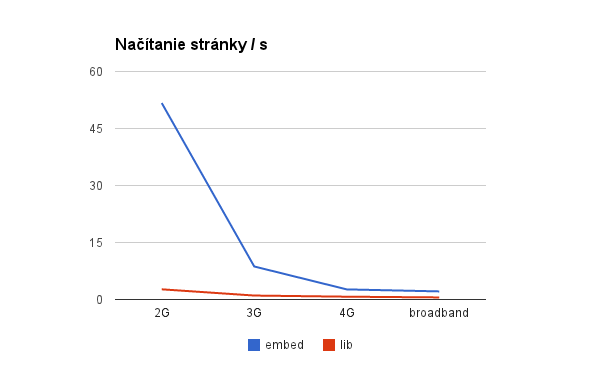
\includegraphics[width=\textwidth]{img/load/youtube-fullload.png}
  \end{subfigure}%
  \begin{subfigure}[b]{0.32\textwidth}
          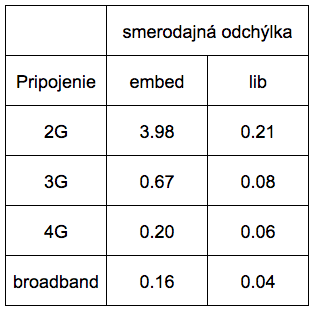
\includegraphics[width=\textwidth]{img/load/y-std-l.png}
  \end{subfigure}%
  % \includegraphics[width=0.6\textwidth]]{img/load/youtube-fullload.png}
  % 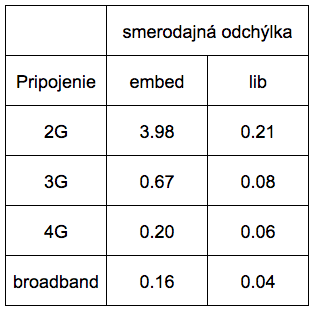
\includegraphics[width=0.4\textwidth]{img/load/y-std-l.png}
  \caption[Porovnanie rýchlosti plného načítania stránky s youtube komponentom]{
    Porovnanie rýchlosti plného načítania stránky s youtube komponentom}
  \label{fig: youtube-fullload}
\end{figure}

Rozdiel v rýchlosti načítania kompletnej stránky aj s externými zdrojmi je veľmi výrazný a pri pomalšom pripojení narastá. Použitím nášho modulu vieme zrýchliť načítanie stránky o sekundy a rozdiel sa prejaví aj pri rýchlejších pripojeniach. Keďže v súčasnosti je na mobilných platformách rozšírené 3G pripojenie, tak sa podstatne zvýši aj použivateľský zážitok, keďže tým ubúda podstatná doba čakania a zároveň používateľom ušetríme aj dáta z predpladtných internetových balíkov.

% \begin{figure}[H]
%   \centering
%   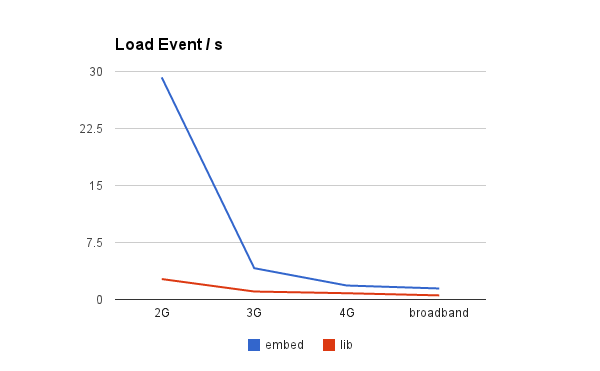
\includegraphics[width=0.6\textwidth]{img/load/youtube-load.png}
%   \caption[Porovnanie rýchlosti load udalosti stránky s youtube komponentom]{
%     Porovnanie rýchlosti load udalosti stránky s youtube komponentom}
%   \label{fig: youtube-load}
% \end{figure}

Použitím nášho modulu sa však zvýši aj čas zostavenia DOM stromu stránky. Nasledujúci graf nie je prekvapením keďže oproti vloženiu videa do stránky potrebujeme ešte načítavať a spúšťať naše skripty. Napriek tejto počiatočnej nevýhode však umožníme výrazné zrýchlenie načítania stránky s youtube videom.

\begin{figure}[H]
  \centering
  \begin{subfigure}[b]{0.6\textwidth}
          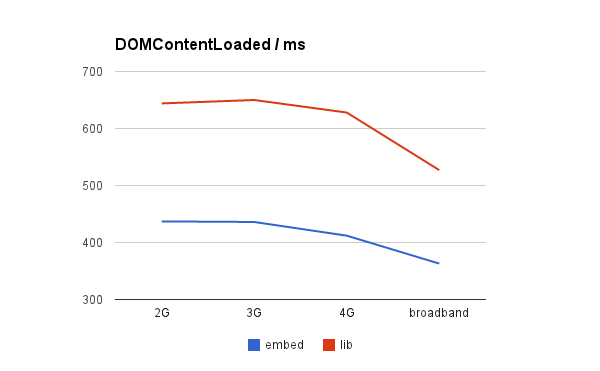
\includegraphics[width=\textwidth]{img/load/youtube-dom.png}
  \end{subfigure}%
  \begin{subfigure}[b]{0.32\textwidth}
          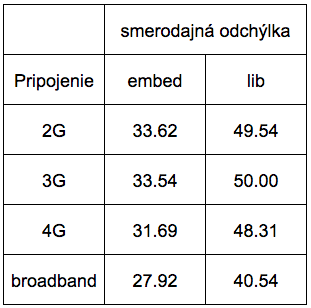
\includegraphics[width=\textwidth]{img/load/y-std-dom.png}
  \end{subfigure}%
  % 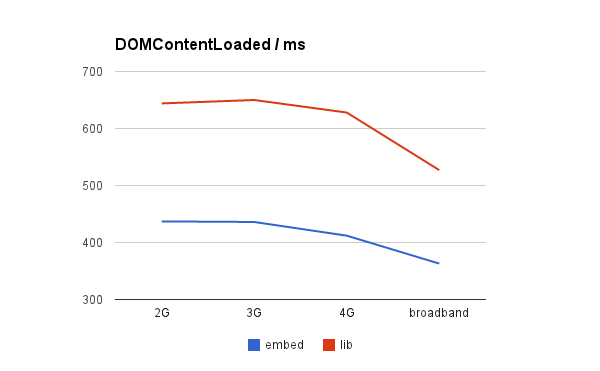
\includegraphics[width=0.6\textwidth]{img/load/youtube-dom.png}
  \caption[Porovnanie rýchlosti zostavenia dom stromu s youtube komponentom]{
    Porovnanie rýchlosti zostavenia dom stromu s youtube komponentom}
  \label{fig: youtube-dom}
\end{figure}


% subsubsection adaptive_youtube (end)

% \newpage
\subsubsection{Modul adaptive-googlemaps} % (fold)
\label{sub:adaptive_googlemaps}

Webový komponent google máp bol demonštrovaný vytvorením modulu adaptive-googlemaps \footnote{\url{https://github.com/angular-adaptive/adaptive-googlemaps}} a demo aplikácie. V aplikácii je umožnené meniť zvýraznené body, centrovanie, priblíženie a zobrazený terén a automaticky sa prispôsobí používateľovmu zariadeniu. Pokiaľ sa pristupuje z mobilného zariadenia a pomalého pripojenia na internet, tak sa zobrazí len náhľad mapy v podobe obrázku. Až po kliknutí na mapu sa dotiahne interaktívna mapa, respektíve mapa sa otvorí v natívnej mobilnej aplikácii. Vytvorená demo aplikácia je znázornená na nasledujúcom obrázku:

\newpage
\begin{figure}[H]
  \centering
  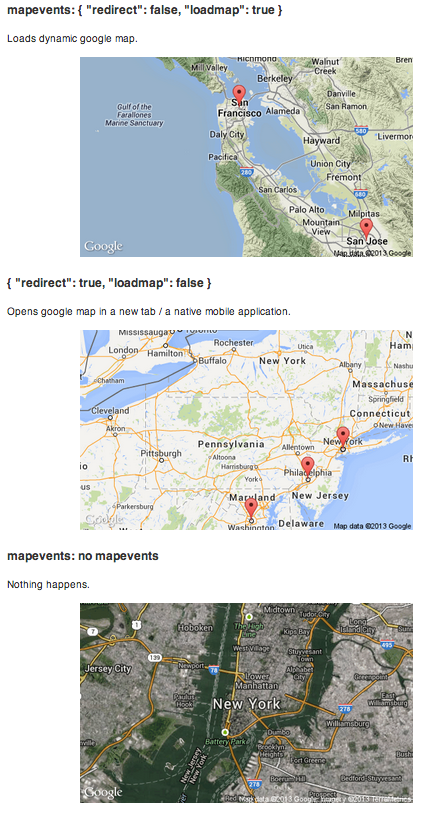
\includegraphics[width=0.5\textwidth]{img/adaptivegooglemaps.png}
  \caption[Prototypová aplikácia vytvoreného modulu adaptive-googlemaps]{
    Prototypová aplikácia vytvoreného modulu adaptive-googlemaps}
  \label{fig: adaptivemotion}
\end{figure}

Použitím vytvoreného modulu vieme opäť ušetriť mnoho dát a znížiť množstvo dopytov na servery. Porovnanie priemerného množstva spotrebovaných dát a vytvorených dopytov pre jeden element google mapy je zobrazené v nasledujúcej tabuľke:

\begin{table}[H]
  \begin{tabular}{ |c|c|c|c| }
    \hline
    & Embed mapa & Vytvorený modul \\ \hline
    Počet požiadaviek na server & 68 & 6 \\  \hline
    Množstvo prenesených dát  & 5540 KB & 476 KB  \\
    \hline
  \end{tabular}
  \caption[Množstvo požiadaviek a prenesených dát pre google mapy]{Množstvo požiadaviek a prenesených dát pre google mapy}
\end{table}

Z toho je zrejme, že použitím vytvoreneho modulu sa opäť zrýchli aj načítavanie webovej stránky. Porovnanie načítavania stránky s použitím klasického prístupu vloženia mapy a použitím nášho modulu a ako sa prejaví zmena rýchlosti na iných druhoch najmä mobilných pripojení je znázornené na nasledujúcom grafe:

\begin{figure}[H]
  \centering
  \begin{subfigure}[b]{0.6\textwidth}
          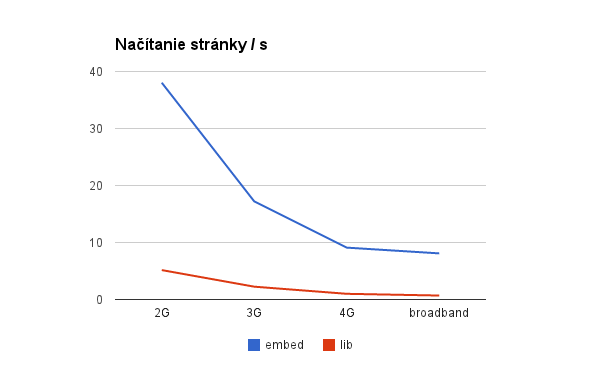
\includegraphics[width=\textwidth]{img/load/gmaps-fullload.png}
  \end{subfigure}%
  \begin{subfigure}[b]{0.32\textwidth}
          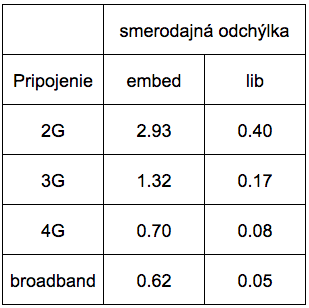
\includegraphics[width=\textwidth]{img/load/gm-std-l.png}
  \end{subfigure}%
  % 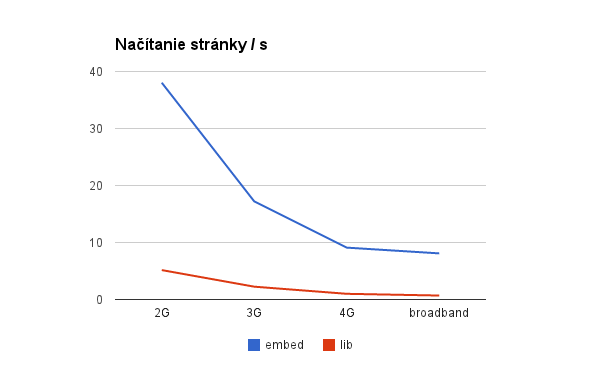
\includegraphics[width=0.6\textwidth]{img/load/gmaps-fullload.png}
  \caption[Porovnanie rýchlosti plného načítania stránky s google maps komponentom]{
    Porovnanie rýchlosti plného načítania stránky s google maps komponentom}
  \label{fig: gmaps-fullload}
\end{figure}

Rozdiel v rýchlosti načítania kompletnej stránky aj s externými zdrojmi je v prípade google mapy ešte výraznejší ako pre zoutube video. Použitím nášho modulu vieme zrýchliť načítanie stránky o sekundy a rozdiel sa prejaví aj pri rýchlejších pripojeniach. Najmä na mobilných pripojeniach sa tým podstatne zvýši aj použivateľský zážitok, keďže tým ubúda podstatná doba čakania a opäť používateľom ušetríme aj dáta z predpladtných internetových balíkov.

% \begin{figure}[H]
%   \centering
%   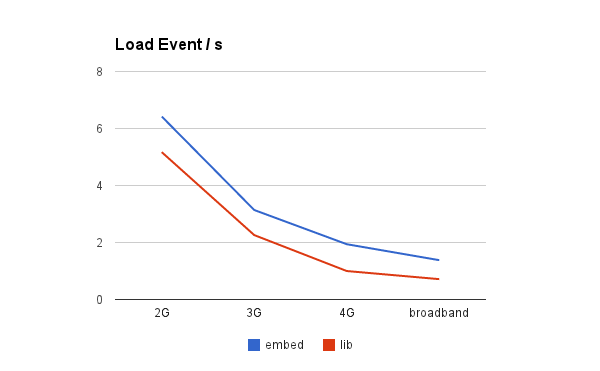
\includegraphics[width=0.6\textwidth]{img/load/gmaps-load.png}
%   \caption[Porovnanie rýchlosti load udalosti stránky s google maps komponentom]{
%     Porovnanie rýchlosti load udalosti stránky s google maps komponentom}
%   \label{fig: gmaps-load}
% \end{figure}

Použitím nášho modulu sa opäť zvýši aj čas zostavenia DOM stromu stránky ako v prípade youtube videa, keďže oproti vloženiu mapy do stránky potrebujeme načítavať a spúšťať naše skripty. Napriek tejto počiatočnej nevýhode však umožníme výrazné zrýchlenie načítania stránky s google mapou.

\begin{figure}[H]
  \centering
  \begin{subfigure}[b]{0.6\textwidth}
          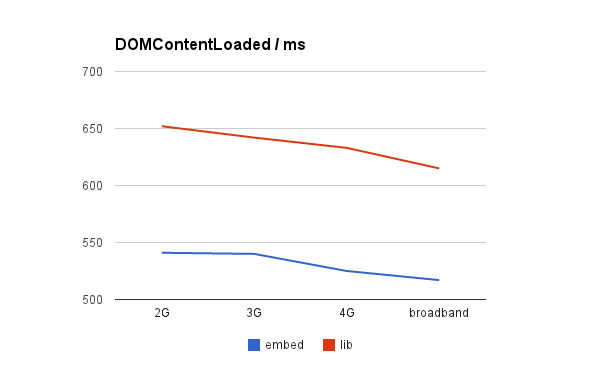
\includegraphics[width=\textwidth]{img/load/gmaps-dom.png}
  \end{subfigure}%
  \begin{subfigure}[b]{0.32\textwidth}
          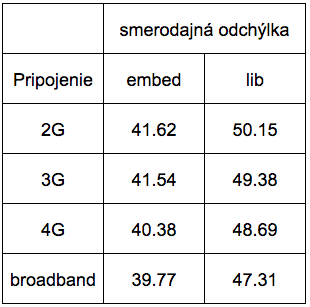
\includegraphics[width=\textwidth]{img/load/gm-std-dom.png}
  \end{subfigure}%
  % 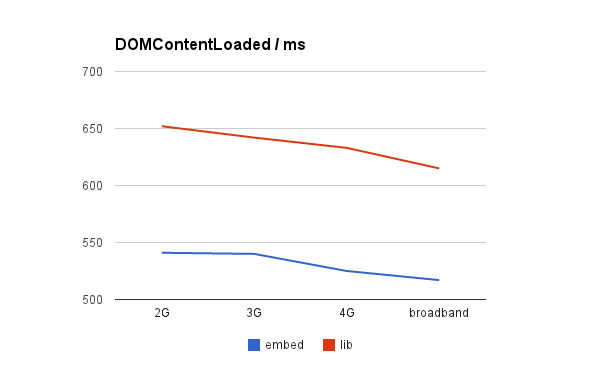
\includegraphics[width=0.6\textwidth]{img/load/gmaps-dom.png}
  \caption[Porovnanie rýchlosti zostavenia dom stromu s google maps komponentom]{
    Porovnanie rýchlosti zostavenia dom stromu s google maps komponentom}
  \label{fig: gmaps-dom}
\end{figure}

% subsubsection adaptive_googlemaps (end)

% subsection webov_komponenty (end)


% subsection  (end)

\newpage
\section{Záver} % (fold)
\label{sec:z_ver}

V práci som navrhol a vytvoril možnosti adaptácie webových aplikácií, či už pomocou alternatívnych možností ovládania rečou, pohybom alebo gyroskopom, prispôsobovaním sa webových komponentov podmienkam používateľa alebo samotných nástrojov použitých pri vývoji adaptívnej webovej aplikácie.

Vytvorené nástroje sú umiestnené na serveri github pod open source licenciou, kde komunita o ne prejavila veľký záujem. Dostal som k nim množstvo pozitívnej spätnej väzby od kvalifikovaný ľudí, pull requestov na drobné úpravy funkcionality či dokumentácie a ďalej sa tak rozvíjajú aj za pomoci ostatných ľudí, za čo by som sa im chcel ešte raz poďakovať. Vďaka tomu som mal možnosť naučiť sa množstvo nových vecí z tvorby open source aplikácií a následne nadobudné poznatky ďalej prezentovať ostatným vývojárom. Zároveň sa referencie na našu prácu objavili v množstve rôznych vydaní newsletterov, konferencií či iných prezentácií:

\begin{itemize}
  \item \textbf{JavaScript Weekly \#135}
  \item \textbf{AngularJS Weekly}
  \item \textbf{deSymfony 2013}, 20-22 jún 2013, Madrid
  \item \textbf{Lone StarPHP 2013}, 28-29 jún 2013, Dallas, TX
  \item \textbf{WebElement \#25}, 5 december 2013, Bratislava
\end{itemize}

\begin{figure}[H]
  \centering
  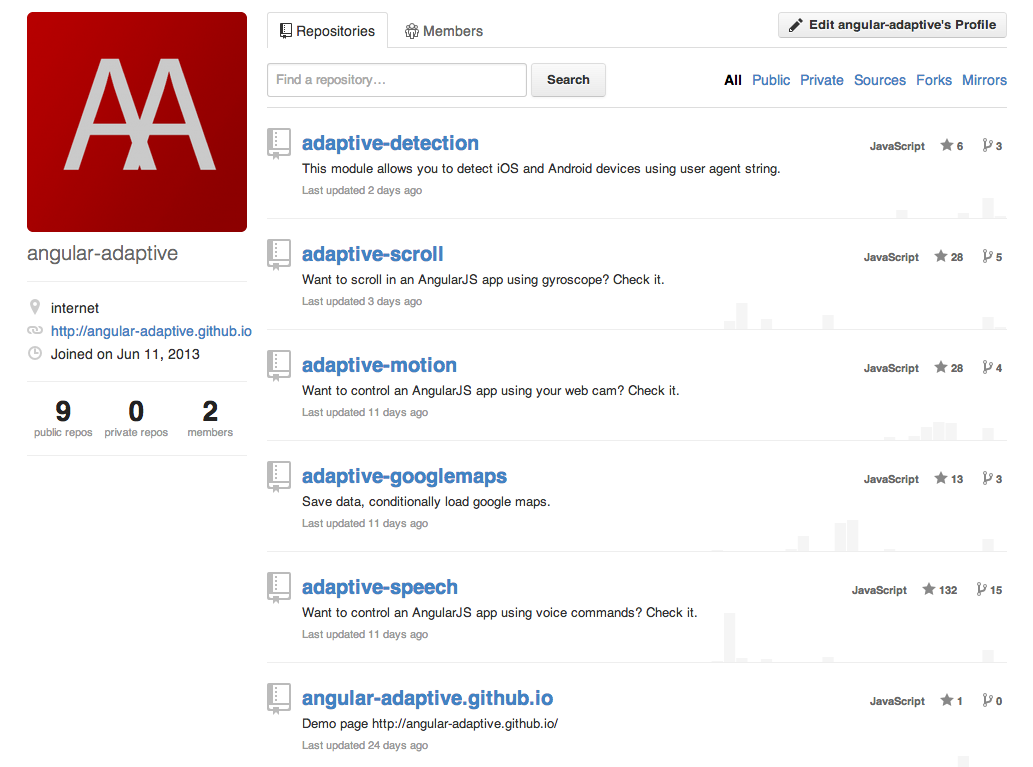
\includegraphics[width=0.7\textwidth]{img/github.png}
  \caption[Umiestnenie projektu na serveri github]{
    Umiestnenie projektu na serveri github\\
    \url{https://github.com/angular-adaptive}}
  \label{fig: github}
\end{figure}

Overením ich používania sa zistilo, že alternatívne spôsoby ovládania sú celkom dobrý doplnok v súčasnosti ku klasickej interakcii so zariadeniami. Tak ako sme očakávali, najpopopulárnejším alternatívnym spôsobom ovládania je ovládanie pomocou reči, nakoľko pomocou neho sa dá kontrolovať celá webová aplikácia len za pomoci rečových príkazov. Ovládania pomocou detakcie pohybu z gyroskopu a video kamery sa tiež presadili, neboli však až na takej úrovni ako ovládanie pomocou reči. Hlavným dôvodom sú výrazne limitované možnosti kde sa dá takéto ovládanie využiť a obe slúžia len ako doplnkový spôsob interakcie. Použitie alternatívneho ovládania je ale aj tak dobrou príležitosťou na zvýšenie používateľského zážitku.

Adaptívne webové komponenty sú dobrý spôsob ako vieme ušetriť množstvo prenášaných dát. Ich použitím sa zrýchlilo načítavanie aplikácie a s tým aj používateľský zážitok. Avšak aj tu existujú limity, nakoľko množstvo webových stránok si potrebuje prispôsobiť webové komponenty vlastným požiadavkam. To preukázal aj nižší záujem z komunity oproti adaptívnym vstupným metódam. Sú však veľmi dôležitou súčasťou webu a verím, že v budúcnosti sa budú takéto spôsoby ešte viac presadzovať.


% section z_ver (end)